\documentclass[11pt,a4paper]{article}
\usepackage[margin=20mm,top=20mm,bottom=20mm,headheight=15pt]{geometry}
\usepackage{fontspec}
\usepackage{amsmath,amssymb,mathtools}
\usepackage{unicode-math}
\setmainfont{Noto Serif CJK SC}[BoldFont={Noto Serif CJK SC Bold},Mapping=tex-text]
\setsansfont{Noto Sans CJK SC}[BoldFont={Noto Sans CJK SC Bold},Mapping=tex-text]
\XeTeXlinebreaklocale "zh"
\XeTeXlinebreakskip=0pt plus 1pt
\renewcommand{\contentsname}{目录}
\setmonofont{Latin Modern Mono}
\setmathfont{Latin Modern Math}
\usepackage{graphicx,xcolor}
\definecolor{Ink}{HTML}{20282D}
\definecolor{Muted}{HTML}{626B70}
\usepackage{longtable,booktabs,array,calc}
\usepackage{caption,float,placeins}
\renewcommand{\topfraction}{0.95}
\renewcommand{\bottomfraction}{0.95}
\renewcommand{\textfraction}{0.05}
\renewcommand{\floatpagefraction}{0.65}
\setlength{\intextsep}{8pt plus 2pt minus 2pt}
\setlength{\textfloatsep}{10pt plus 2pt minus 2pt}
\setlength{\floatsep}{10pt plus 2pt minus 2pt}
\usepackage{enumitem,fancyhdr,titlesec}
\usepackage{needspace}
\usepackage{microtype}
\usepackage{xurl}
\usepackage[unicode,hidelinks,breaklinks]{hyperref}
\hypersetup{pdftitle={认知预测地图中方向与时间权重的机制识别},pdfauthor={Yongzhang
Ji},pdfsubject={SR mechanism identification, experimental design and joint measurement uncertainty},pdfkeywords={successor representation, cognitive maps, identifiability, qualitative properties, temporal direction}}
\setlength{\parindent}{0pt}
\setlength{\parskip}{5pt plus 1pt minus 1pt}
\linespread{1.12}
\lefthyphenmin=3
\righthyphenmin=3
\hyphenpenalty=1500
\exhyphenpenalty=1500
\setlength{\emergencystretch}{3em}
\setcounter{secnumdepth}{0}
\setcounter{tocdepth}{2}
\raggedbottom
\widowpenalty=10000
\clubpenalty=10000
\displaywidowpenalty=10000
\allowdisplaybreaks[1]
\predisplaypenalty=10000
\postdisplaypenalty=1000
\titleformat{\section}{\sffamily\bfseries\Large\color{Ink}}{}{0em}{}
\titleformat{\subsection}{\sffamily\bfseries\normalsize\color{Ink}}{}{0em}{}
\titleformat{\subsubsection}{\sffamily\bfseries\normalsize}{}{0em}{}
\titlespacing*{\section}{0pt}{17pt plus 3pt}{7pt}
\titlespacing*{\subsection}{0pt}{12pt plus 2pt}{5pt}
\titlespacing*{\subsubsection}{0pt}{10pt plus 2pt}{4pt}
\setlist{nosep,leftmargin=1.5em}
\setlist[enumerate]{itemsep=3pt}
\providecommand{\tightlist}{\setlength{\itemsep}{0pt}\setlength{\parskip}{0pt}}
\providecommand{\passthrough}[1]{#1}
\makeatletter
\def\maxwidth{\ifdim\Gin@nat@width>\linewidth\linewidth\else\Gin@nat@width\fi}
\def\maxheight{\ifdim\Gin@nat@height>0.56\textheight0.56\textheight\else\Gin@nat@height\fi}
\makeatother
\setkeys{Gin}{width=\maxwidth,height=\maxheight,keepaspectratio}
\pagestyle{fancy}
\fancyhf{}
\fancyhead[L]{\sffamily\footnotesize\color{Muted} 认知预测地图的机制识别}
\fancyhead[R]{\sffamily\footnotesize\color{Muted} 预印本}
\fancyfoot[C]{\sffamily\footnotesize\color{Muted}\thepage}
\renewcommand{\headrulewidth}{0pt}
\renewcommand{\footrulewidth}{0pt}
\begin{document}
\thispagestyle{plain}
{\raggedright\hyphenpenalty=10000\sffamily\bfseries\color{Ink}\fontsize{20}{25}\selectfont 认知预测地图中方向与时间权重的机制识别\par}
\vspace{8pt}
{\sffamily\fontsize{12}{15}\selectfont Yongzhang Ji\par}
\vspace{4pt}
{\sffamily\small Faculty of Psychology, Southwest University, Chongqing,
China\par}
\vspace{3pt}
{\sffamily\footnotesize\color{Muted} ORCID: \href{https://orcid.org/0009-0006-4111-2000}{0009-0006-4111-2000}\par}
\vspace{7pt}
{\sffamily\footnotesize\color{Muted} 预印本\quad |\quad 2026-11-26\par}
\vspace{8pt}
\section{摘要}\label{ux6458ux8981}

继任表征（successor
representation，SR）提出，当前状态可以通过未来状态的折扣占据来表示。把这种关系用于解释神经数据，需要分别确定表征的时间方向与时间权重。我们从状态转移和神经观测出发，研究连续
SR
模型族中哪些性质能够被识别。规范欧氏几何可使方向相反的地图完全相同；已学习参考甚至可以使两个前瞻条件在完整状态对比空间中的相对作用等于一个后瞻
SR。连续族分析将这些等价统一为相容解释集合的问题，并揭示方向与参数具有不同的信息要求：在直接参考的单旋转平面中，方向可以确定，而任意折扣仍可由当前与预测权重补偿。互反任务在完整
SR
及指定扩展族中形成方向排他区域，任务相容读出保留这些关系，联合误差反演支持有限样本中的性质声明。相对角度已经给出尖锐折扣范围；进一步增加独立传播形状，可以确定参数的唯一值或有限时间核。有限记忆设计还允许检验多尺度混合，并在参考已经学习时恢复目标核的相对形状。公开重复神经测量显示，任务相关参考具有预测收益，恰当的误差空间和读出增加了已知变换的可判断情境，真实采集层级则决定这些判断的可迁移范围。这些结果给出一条从观测相容性走向机制性质、再走向定量约束的研究路径。

\textbf{关键词：}
继任表征；认知地图；可辨识性；预测方向；时间权重；连续模型族

\section{引言}\label{ux5f15ux8a00}

当我们来到熟悉的路口，眼前的景象并不是全部信息。我们知道刚才从哪里来，也知道沿不同方向走下去会遇见什么。认知地图将这些关系带入当前的行为：记住过去有助于辨认情境，预期未来有助于规划行动。两种计算使用的可能是同一组地点或事件，区别在于它们如何围绕现在组织起来。

继任表征为其中的前瞻关系给出了一个具体模型
{[}1{]}。它把当前状态表示为从这里出发、未来可能占据的各状态的带权总和。预测地图理论将这一思想用于海马群体表征，并解释状态转移与表征相似性之间的联系
{[}2{]}。这一研究方向随后延伸到抽象关系、跨区域预测时域、序列预期与学习后的表征变化
{[}5–8,19{]}。这些现象使一个机制问题变得重要：当神经活动包含与未来有关的结构时，我们能够由此确定系统怎样组织时间吗？

这个问题有两个相互关联的部分。首先是方向：当前表征包含即将经历的状态、刚刚经历的状态，还是二者的混合？其次是权重：不同时间距离怎样进入当前表征，它们是否服从同一个几何折扣？已有研究为区分这些可能性提供了多种路径。时间情境与
SR 的关系揭示了某些学习条件下的机制等价
{[}3{]}；重估实验利用参与者能够重新获得的信息区分规划过程
{[}4{]}；基率、图结构与查询要求可以使前后预测产生不同的行为选择
{[}9{]}；多尺度表征与对称学习规则则扩大了可供研究的机制范围
{[}10,11{]}。

神经测量为这个问题增加了另一层关系。我们通常记录多个来源混合后的模式，再比较模式间距离，或者借助参考测量读出其内容。表征模型的研究已经说明，特征基、先验与测量方式共同规定了经验预测
{[}12–14{]}。因此，一种机制能否被识别，既取决于它怎样生成内部表征，也取决于哪些差异能够保留到研究者实际使用的观测中。对
SR 而言，状态转移、时间权重与参考本身的学习结构会在这里共同发挥作用。

本文沿着这一关系展开。我们先用两个精确例子说明，不同方向如何在距离几何或已学习参考的相对作用中重合。随后考察全部合法参数产生的连续预测族，询问同一观测留下的所有解释是否共享某种性质。这个问题使方向判断与参数恢复可以分别研究：参数可能仍沿连续曲线变化，而方向已经确定。互反任务、任务相容读出和联合误差将这一原则落实为可执行的推断；更多独立传播信息则继续支持折扣和时间核的定量识别。真实重复神经测量最后检验这条路径中的参考、读出与采集要求。

\section{结果}\label{ux7ed3ux679c}

\Needspace{7\baselineskip}
\subsection{1.
预测地图的两个机制问题}\label{ux9884ux6d4bux5730ux56feux7684ux4e24ux4e2aux673aux5236ux95eeux9898}

\Needspace{6\baselineskip}
\subsubsection{1.1
从状态转移到未来占据}\label{ux4eceux72b6ux6001ux8f6cux79fbux5230ux672aux6765ux5360ux636e}

每天从家去办公室，我们会经过路口、车站，也可能顺路到商店。站在路口时，我们知道自己在哪里，也知道从这里继续走，哪些地方更可能出现在接下来的经历中。继任表征（successor
representation，SR）将后一种关系写进了当前状态的表征。它所表达的问题是：“从这里出发，我未来可能经历什么？”

SR 最初由 Dayan 在 1993
年的强化学习研究中提出，用后继状态之间的关系组织表征，以提高长期回报预测的效率
{[}1{]}。理解这个模型，可以从一步转移开始。设 \(P_{ij}\) 是当前位于状态
\(i\) 时，下一步到达状态 \(j\) 的概率。转移矩阵 \(P\)
的每一行都描述从一个状态出发的去向。例如，从路口下一步到车站的概率为
\(0.75\)，到商店的概率为
\(0.25\)；从车站和商店下一步到办公室的概率分别为 \(0.8\) 和
\(0.4\)。那么，从路口经过两步到办公室的概率，就是两条可能路线的概率之和：\(0.75\times0.8+0.25\times0.4=0.70\)。

\par
\noindent\begin{minipage}{\linewidth}

矩阵乘法把这种“先经过哪里，再到哪里”的计算同时用于所有状态：

\[
(P^2)_{ik}=\sum_jP_{ij}P_{jk}.
\]

\end{minipage}\par

因此，\(P\) 给出一步后的分布，\(P^2\) 给出两步后的分布，\(P^3\)
给出三步后的分布。这里的幂表示连续转移；每一次相乘都对所有可能的中间状态求和。给定稳定的任务或行为策略，我们便可以从一步转移逐渐展开未来。

\par
\noindent\begin{minipage}{\linewidth}

为了将这些不同距离的未来合成一个当前表征，SR 为第 \(t\) 步赋予权重
\(\gamma^t\)。我们考虑持续进行的有限状态任务，取 \(0\leq\gamma<1\)，得到

\[
M_\gamma(P)=I+\gamma P+\gamma^2P^2+\gamma^3P^3+\cdots.
\]

\end{minipage}\par

其中，\(I\) 表示当前状态，\(\gamma P\)
表示一步后的加权分布，\(\gamma^2P^2\) 表示两步后的加权分布。\(\gamma\)
越大，较远未来在当前表征中保留的权重越多。矩阵的一行描述从某个当前状态出发，对所有状态的折扣占据预测。同一个状态可能在许多未来步长被再次到访，所以这一行是跨时间的占据总和，其总量可以大于一。

\par
\noindent\begin{minipage}{\linewidth}

这个级数还有一个简洁的写法。将它乘以 \(\gamma P\)，得到从 \(\gamma P\)
开始的同一串后续项；从原式中减去，后续项依次抵消，只留下 \(I\)。于是

\[
(I-\gamma P)M_\gamma=I,
\qquad
M_\gamma(P)=(I-\gamma P)^{-1}.
\]

\end{minipage}\par

逆矩阵因此是多步占据累加的简写。它描述表征之间应满足的关系，学习系统可以通过逐步更新接近这种关系。若各状态的即时奖励组成向量
\(r\)，那么 \(V=M_\gamma r\)
将未来占据预测转化为长期价值预测。预测状态与评估这些状态的奖励由此可以分别组织。

Stachenfeld、Botvinick 和 Gershman 将这一结构发展为海马的预测地图理论
{[}2{]}。按照这种解释，当前的群体神经活动除了包含当前位置，还包含可能到访状态的信息。两个地点即使空间相隔较远，只要它们预示着相似的未来，也可能具有相似的群体表征。这使
SR 成为连接学习、认知地图与神经表征的一种具体假说。

\Needspace{6\baselineskip}
\subsubsection{1.2
认知地图的方向与权重}\label{ux8ba4ux77e5ux5730ux56feux7684ux65b9ux5411ux4e0eux6743ux91cd}

当一个表征包含了当前状态以外的信息，我们还需要问，这些信息来自哪个时间方向。在路口的表征中，家的信息可以来自刚刚经历的路径，车站的信息可以来自即将到达的地方。一个机制可以向前整合，一个机制可以向后整合，也可以将两者结合。有关时间情境、预测层级和多步预期的研究，使这些可能性都具有明确的认知意义
{[}3,6,8,9,11{]}。

\par
\noindent\begin{minipage}{\linewidth}

为了将方向写清楚，前瞻模型使用从现在到未来的转移
\(P\)；后瞻模型使用给定现在时，过去状态的条件分布。若任务处于平稳分布
\(\pi\)，正确的后向转移为

\[
P^*=D_\pi^{-1}P^\top D_\pi,
\]

\end{minipage}\par

其中 \(D_\pi\)
的对角元素是各状态出现的平稳概率。这一加权反映一个简单事实：较常出现的状态，也可能较常成为某个当前状态的来源。在均匀平稳任务中，所有状态的出现频率相同，便有
\(P^*=P^\top\)。我们先用这类任务建立直觉，非均匀情形的观测坐标与度量在方法及补充材料中给出。

另一个问题是时间权重。即使数据已经支持未来信息，也还需要确定这些信息如何结合。SR
采用 \(1,\gamma,\gamma^2,\ldots\)
的几何规则，将当前反应、一步预测和更远预测联系在一起。这是一项有明确内容的模型约束。当前状态的感觉反应可以独立改变，未来信息的总增益也可以改变；同一群体还可能混合多个预测时域。

\par
\noindent\begin{minipage}{\linewidth}

这种区别可以用一个稍大的模型族表示。令

\[
N_\gamma(P)=P+\gamma P^2+\gamma^2P^3+\cdots
=P(I-\gamma P)^{-1},
\]

\end{minipage}\par

并考虑 \(G(P)=cI+\alpha N_\gamma(P)\)。这里 \(c\)
决定当前成分，\(\alpha\) 决定未来传播的总强度，\(\gamma\)
决定未来各步之间的相对权重。缩放后的完整 SR，\(aM_\gamma(P)\)，恰好满足
\(c=a\)、\(\alpha=a\gamma\)。其中 \(N_0(P)=P\) 仍保留一步预测，而完整 SR
的 \(M_0(P)=I\) 只有当前成分。所以完整 SR
是这个更大族中具有特定绑定关系的一部分。后文将看到，解除这项绑定会改变数据能够确定的内容。

本文由此集中考察两项机制承诺：表征指向什么时间方向，以及不同时间距离具有怎样的权重。它们允许不同精度的回答。数据可能已经确定方向，却仍兼容多个时域；也可能同时限制方向和一部分参数范围。我们从这些可以分别检验的问题出发，逐步建立更具体的机制解释。

\Needspace{6\baselineskip}
\subsubsection{1.3
神经记录如何承载这些关系}\label{ux795eux7ecfux8bb0ux5f55ux5982ux4f55ux627fux8f7dux8fd9ux4e9bux5173ux7cfb}

\par
\noindent\begin{minipage}{\linewidth}

数学模型以状态作为坐标，实验测量却通常以神经元、体素或电极作为坐标。一根电极不会自动告诉我们，它记录的是车站、办公室，还是几个来源的共同活动。为了连接两者，将状态平均模式写为

\[
Y=G(P)B+E.
\]

\end{minipage}\par

\(Y\) 的行对应状态，列对应记录通道；\(B\)
表示状态成分怎样映入这些通道，\(E\) 表示测量误差。\(G(P)\)
则规定当前、过去和未来的信息如何在状态之间传播。在比较多个实验条件时，共同的
\(B\)
表示条件间保持同一套基础神经映射。正整体增益、共同状态偏置和非均匀状态权重在方法中一并处理（补充材料
T01）。

这使研究问题更加具体：两种机制在内部的计算不同，它们经过实际测量之后，是否仍然留下不同的关系？我们先从一种常用的观测摘要开始。即使暂时没有测量误差，机制差异也可能在这一步消失。

\Needspace{7\baselineskip}
\subsection{2.
不同机制产生相同观测的两种精确困难}\label{ux4e0dux540cux673aux5236ux4ea7ux751fux76f8ux540cux89c2ux6d4bux7684ux4e24ux79cdux7cbeux786eux56f0ux96be}

\Needspace{6\baselineskip}
\subsubsection{2.1
从活动模式到表征距离}\label{ux4eceux6d3bux52a8ux6a21ux5f0fux5230ux8868ux5f81ux8dddux79bb}

\par
\noindent\begin{minipage}{\linewidth}

假设在地点 A 和 B 记录到以下活动模式：

\[
x_A=(1,0.7,0.4),\qquad x_B=(1,0.6,0.5).
\]

\end{minipage}\par

\par
\noindent\begin{minipage}{\linewidth}

它们比较相似。另一个地点 C 的模式为

\[
x_C=(0.1,0.2,1.5),
\]

\end{minipage}\par

看起来与 A 相差较大。研究者于是可以问：A 和 B
的相似，是否因为它们预示着相似的未来，而 C 预示着不同的未来？

\par
\noindent\begin{minipage}{\linewidth}

表征相似性分析使这类问题可以定量比较
{[}12{]}。例如，两个模式的平方欧氏距离为

\[
d(A,B)^2=\sum_j(x_{Aj}-x_{Bj})^2.
\]

\end{minipage}\par

在这个说明性例子中，\(d(A,B)^2=0.02\)，\(d(A,C)^2=2.27\)。对所有状态两两计算，就得到表征距离矩阵（representational
dissimilarity
matrix，RDM）。模型可以预测哪些状态应当接近，哪些应当分离，再与神经数据中的距离结构比较。

这一步将完整神经活动向量压缩成了状态之间的距离。若把所有向量一起旋转，甚至作镜像反射，彼此距离都会保持不变。因此，相同
RDM
可以对应不同的坐标关系。预测地图的方向是否会恰好落入这种不变性，是一个需要单独回答的问题。

\par
\noindent\begin{minipage}{\linewidth}

我们在以任务状态为特征的规范坐标中得到精确答案。设 \(P\)
为双随机转移矩阵，即每行和每列均为一，前后 SR 使用同一个非零折扣
\(0<\gamma<1\)。那么，完整欧氏行距离满足

\[
\operatorname{RDM}\{M_\gamma(P)\}
=\operatorname{RDM}\{M_\gamma(P^\top)\}
\quad\Longleftrightarrow\quad
PP^\top=P^\top P.
\]

\end{minipage}\par

右侧条件称为正规性。它允许转移具有很强的方向。例如，沿一个有向环不断前进，与沿同一环反向前进，显然是两种不同的路径；但这些转移可以满足上述条件。由它们构成的前后预测地图，仍具有完全相同的状态间距离（图
1；补充材料 T02）。

这个结果也说明，几何中的方向缺失并不要求行为过程接近无方向。在有向环上，可以让反向边的概率越来越小，使过程的不可逆性不断增强，同时保持所有合法折扣下的前后几何等价。多个相互独立的旋转块还能形成多组带标签方向不同、几何相同的任务（补充材料
T03）。完整证明进一步用 \(PP^\top-P^\top P\) 给出几何差异的上下界。

这一关系刻画了规范欧氏观测的识别边界。实验中的其他特征度量、神经混合和部分状态观测，可以按照各自的观测映射继续分析。重要的起点是，方向明确的任务不一定把方向信息留在两两距离中。相似性与预测地图相符时，我们还需要知道哪些竞争机制具有同样的相似性。

\Needspace{6\baselineskip}
\subsubsection{2.2
保留完整模式后，参考为何重要}\label{ux4fddux7559ux5b8cux6574ux6a21ux5f0fux540eux53c2ux8003ux4e3aux4f55ux91cdux8981}

一个自然的下一步，是保留完整模式，寻找距离摘要没有保留的作用关系。但完整模式仍然经过了未知的神经映射。在
\(Y=MB\) 中，单次观测同时包含 \(M\) 与
\(B\)；改变机制，也可以改变与它相配的映射。使用参考测量的目的，是给这种分解提供一个共同基准。

最直接的情形，是参考模式给出 \(B\)，目标模式给出
\(MB\)。两者经过同一套记录通道，因而能够询问：目标相对于基准发生了怎样的状态传播？当参考包含恢复所需作用的信息时，可以得到机制的相对算子。这里的“算子”就是把一个模式变成另一个模式的规则。它保留坐标之间怎样结合的信息，比两两距离更为丰富。

参考的科学含义因此很关键。一个直接参考可以锚定基础状态模式；一个已经学习过相关转移的参考，则会将自身的预测结构带入比较。两者都能提供清晰、可重复的记录，但它们定义了不同的推断对象。

\par
\noindent\begin{minipage}{\linewidth}

为把这一点写清楚，我们先消去所有状态共同的平均成分。剩下的坐标描述状态之间的区别，称为状态对比。令
\(A\) 表示任务在这些坐标中的作用，目标和参考分别具有前向 SR
\(M_\gamma(A)\) 与
\(M_\eta(A)\)。若两者共享神经映射，且所需相对作用可见，则得到

\[
T=aM_\gamma(A)M_\eta(A)^{-1},\qquad a>0,
\]

\end{minipage}\par

其中 \(a\) 为整体增益之比。恢复到的是两个学习过程之间的关系。

\Needspace{6\baselineskip}
\subsubsection{2.3
已学习参考可以形成完整的方向别名}\label{ux5df2ux5b66ux4e60ux53c2ux8003ux53efux4ee5ux5f62ux6210ux5b8cux6574ux7684ux65b9ux5411ux522bux540d}

\par
\noindent\begin{minipage}{\linewidth}

同一任务上的两个前向 SR
可以具有不同预测时域。对上述相对算子，代数整理给出

\[
T=a\{I+(\gamma-\eta)A(I-\gamma A)^{-1}\}.
\]

\end{minipage}\par

方向性因此与两个时域的相对关系相连。用任务中带方向的部分构造标记时，直接参考下的前向作用给出正号；同图已学习参考下，这个标记的符号变为
\(\gamma-\eta\) 的符号（补充材料
T04）。目标向前预测得较近，参考向前预测得较远，就可以出现后向的相对标记。两个条件的内部方向都向前，而比较显示的是它们之间的差别。

\par
\noindent\begin{minipage}{\linewidth}

这种现象还可以达到比符号反转更强的程度。我们构造一个七状态任务：从每个状态出发，以相同概率向前移动
1、2 或 4 个编号。它的全部六维状态对比空间允许如下精确关系：

\[
M_{0.3}(A)M_{0.8}(A)^{-1}
=aM_\beta(A^\top),
\]

\end{minipage}\par

其中
\(a=634/519\)、\(\beta=75/173\)，都是合法的正增益和折扣参数。左侧由两个前向、时域不同的学习条件产生；右侧是后向
SR。相等发生在整个六维对比算子上，所以每一个由该算子确定的状态对比预测都相同（图
1；补充材料 T04）。

我们将不同机制在指定观测中精确相同的情形称为别名。这里有两条不同的路径：几何别名来自活动模式到距离的压缩；学习参考别名则发生在保留相对算子之后，因为参考已经成为所比较机制的一部分。前者提醒我们检查摘要保留了什么，后者提醒我们检查基准定义了什么。

精确别名也区分了两种实验困难。噪声造成的不确定性可以随着有效重复测量增加而缩小；两个解释在既定观测层完全相同，则会随着精度提高而趋向同一个结果。要取得新的机制信息，需要增加任务、参考或读出之间的约束。这使接下来的问题从“怎样把这个量估得更准”，推进到“哪些机制性质已经由这个量确定，以及怎样使更多性质能够确定”。

\begin{figure}[!htbp]
\centering
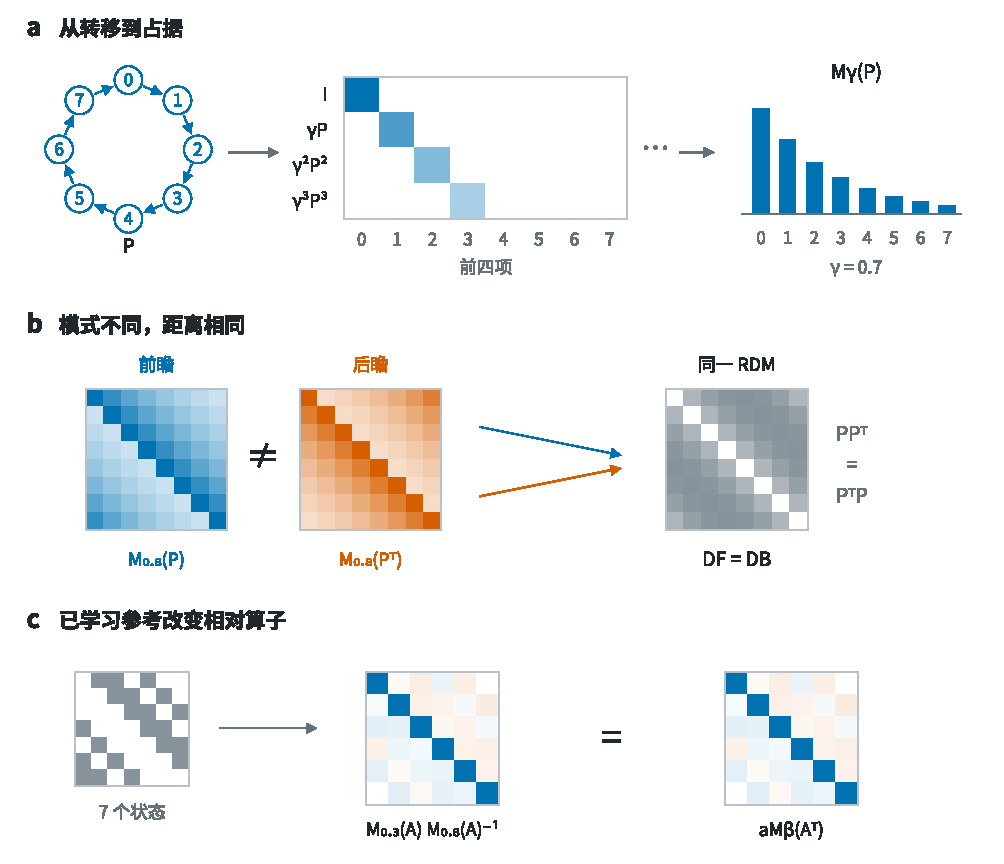
\includegraphics[width=\linewidth,height=0.64\textheight,keepaspectratio]{figures/pdf/fig01_foundations_zh.pdf}
\vspace{3pt}
\begin{minipage}{\linewidth}
\fontsize{9.2}{11.7}\selectfont
\setlength{\parskip}{3pt}

\textbf{图 1. 预测占据与两种精确观测等价。}
\textbf{a，}八状态有向环说明逐步转移如何形成预测地图。中间矩阵显示
\(\gamma=0.7\) 时 \(I,\gamma P,\gamma^2P^2,\gamma^3P^3\) 的状态 0
行；右侧柱高正比于完整 \((I-\gamma P)^{-1}\) 的状态 0
行，包括更晚再次绕回各状态的贡献。\textbf{b，}折扣为 \(0.8\) 时，前后向
SR
的矩阵元素不同，两两欧氏行距离却完全相同，右侧显示共同距离矩阵。在双随机
\(P\)、规范状态特征、同一非零折扣和全部状态对下，距离相等当且仅当
\(PP^\top=P^\top P\)。有向环具有转移箭头，同时也是正规矩阵。\textbf{c，}七状态任务从
\(i\) 等概率转向模七的
\(i+1,i+2,i+4\)。在全部六个正交状态对比上，任务作用 \(A\) 满足
\(M_{0.3}(A)M_{0.8}(A)^{-1}=aM_\beta(A^\top)\)，其中
\(a=634/519\)、\(\beta=75/173\)。因此，两个已学习前向表征可以产生与缩放后瞻
SR
完全相同的相对对比算子。定义状态对比时已去除共同常数方向。热图来自确定性矩阵计算；有符号热图中的蓝、橙分别表示正、负系数。一般结果见补充定理
T02–T04。

\end{minipage}
\end{figure}

\Needspace{7\baselineskip}
\subsection{3.
从全部相容解释中确定机制性质}\label{ux4eceux5168ux90e8ux76f8ux5bb9ux89e3ux91caux4e2dux786eux5b9aux673aux5236ux6027ux8d28}

\Needspace{6\baselineskip}
\subsubsection{3.1
连续预测族把反例变成完整的识别问题}\label{ux8fdeux7eedux9884ux6d4bux65cfux628aux53cdux4f8bux53d8ux6210ux5b8cux6574ux7684ux8bc6ux522bux95eeux9898}

一对精确反例告诉我们，某两个解释会混淆。但读者还会希望知道，混淆占据多大范围，是否存在能够作出判断的区域。为此，我们让机制的折扣、增益以及允许的参考参数遍历整个合法范围，考察它们产生的全部观测。一个机制名称于是对应一个连续预测集合，而不只是一次拟合得到的点。

\par
\noindent\begin{minipage}{\linewidth}

记一个完整解释为
\(\theta\)。它包括机制方向、数值参数和允许变化的测量因素。给定实验及读出，\(\Phi(\theta)\)
表示这个解释产生的观测。对于实际观测 \(y\)，定义

\[
\mathcal C(y)=\{\theta:\Phi(\theta)=y\}.
\]

\end{minipage}\par

这个相容集合保留了所有能够解释同一观测的候选。若我们关心的性质记为
\(q(\theta)\)，例如前后方向、净方向或某个参数范围，那么问题变为：\(\mathcal C(y)\)
中的解释，对这个性质是否一致？

\par
\noindent\begin{minipage}{\linewidth}

这给出一条一般的识别原则：性质能够由观测确定，当且仅当产生同一观测的解释共享这个性质。全局形式为

\[
\Phi(\theta_1)=\Phi(\theta_2)
\Longrightarrow
q(\theta_1)=q(\theta_2).
\]

\end{minipage}\par

它的理由很直接。若同一观测仍兼容相反性质，一个只读取该观测的判断规则，在两种真实机制下会得到相同输入，无法保证两者都判对。若所有相容解释的性质一致，那么选择其中任意一个读取该性质，答案都会相同；这个答案就由观测确定。这是一般可辨识性的标准原则，我们将它用于求出具体
SR 连续族的重合范围和可区分部分（补充材料 T05）。

前面的几何和参考别名由此获得共同解释：观测保留了多个方向不同的候选。另一方面，某个参数不能唯一确定，也可能只是因为相容集合包含了一条参数变化曲线，而曲线上的解释仍共享同一方向。我们接下来展示这种情形。它使定性性质具有独立的、可以精确证明的地位。

\Needspace{6\baselineskip}
\subsubsection{3.2
方向可以确定，而折扣可以连续改变}\label{ux65b9ux5411ux53efux4ee5ux786eux5b9aux800cux6298ux6263ux53efux4ee5ux8fdeux7eedux6539ux53d8}

\par
\noindent\begin{minipage}{\linewidth}

先考虑一个很容易画出的任务作用。将环形任务的状态模式沿两条预先规定的对比轴概括，一步转移在这两条轴上相当于逆时针旋转
\(90^\circ\)。记

\[
J=\begin{pmatrix}0&-1\\1&0\end{pmatrix},\qquad J^2=-I.
\]

\end{minipage}\par

这两条轴描述状态之间的区别。它们可以由许多神经通道共同测得，并不要求存在两颗专门负责旋转的神经元。一个具体的八状态实现将在下节给出。

\par
\noindent\begin{minipage}{\linewidth}

在合格直接参考下，考察当前与未来贡献能够独立变化的模型。状态对比中的当前系数
\(c\) 取实数，预测增益 \(\alpha\geq0\)，折扣
\(0\leq\gamma<1\)。前向作用为

\[
G_+=cI+\alpha J(I-\gamma J)^{-1}=uI+vJ,
\]

\end{minipage}\par

\par
\noindent\begin{minipage}{\linewidth}

其中

\[
u=c-\frac{\alpha\gamma}{1+\gamma^2},\qquad
v=\frac{\alpha}{1+\gamma^2}.
\]

\end{minipage}\par

\(u\) 是沿原方向的贡献，\(v\)
是沿已知任务旋转方向的贡献。让全部合法参数变化，前向族恰好覆盖
\(v\geq0\) 的半平面；同一任务的后向模型使用时间反转作用
\(-J\)，其预测族恰好覆盖 \(v\leq0\) 的半平面（图 2；补充材料
T06）。因此，当 \(v\) 非零且可见时，方向在这一扩展族内已经确定。\(v=0\)
是两族共享的当前成分边界。

\par
\noindent\begin{minipage}{\linewidth}

折扣却具有不同的地位。对每个 \(0\leq\gamma<1\)，选择

\[
c=1+\gamma,\qquad \alpha=1+\gamma^2,
\]

\end{minipage}\par

\par
\noindent\begin{minipage}{\linewidth}

都会得到

\[
G_+=I+J.
\]

\end{minipage}\par

例如，\(\gamma=0\) 时，\(c=1\)、\(\alpha=1\)；\(\gamma=0.5\)
时，\(c=1.5\)、\(\alpha=1.25\)。两个模型的当前贡献和未来衰减不同，最后产生的作用完全一样。连续改变折扣，就得到一整条这样的等价曲线。

于是，同一份观测可以告诉我们，这个作用具有前向性质，却无法在这条曲线上选出唯一折扣。即使观测已经精确到没有误差，这个区别仍然存在。对于落在完整
SR
合法预测范围内的观测，将当前与未来权重绑定会缩小相容集合，甚至给出唯一参数。这样的参数精度因此同时依赖数据与绑定规则。

这个例子将一般模型和特殊模型之间的关系具体化了。一个模型的数值可以拟合得很确定，同时在放宽其他合法权重后失去唯一性；方向这样的性质，却仍可能在扩大的集合中保持不变。性质识别由此给出一种能够跨越参数变化的科学断言。

\Needspace{6\baselineskip}
\subsubsection{3.3
多尺度表征也可以具有单折扣的外观}\label{ux591aux5c3aux5ea6ux8868ux5f81ux4e5fux53efux4ee5ux5177ux6709ux5355ux6298ux6263ux7684ux5916ux89c2}

\par
\noindent\begin{minipage}{\linewidth}

这一平面还带来另一个结果。假设同一神经映射承载多个前向
SR，尺度权重均非负，并允许额外的非负当前成分。它们的总作用为

\[
H(J)=r_0I+\int M_\gamma(J)\,\mu(d\gamma),
\qquad r_0\geq0,\quad\mu\geq0.
\]

\end{minipage}\par

\par
\noindent\begin{minipage}{\linewidth}

在这个平面上，所有成分都可以写成
\(uI+vJ\)。相加后仍然只有这两个系数，因此只要总作用非零，就可以精确写成

\[
H(J)=a_{\mathrm{eff}}M_{\gamma_{\mathrm{eff}}}(J),
\qquad \gamma_{\mathrm{eff}}=v/u.
\]

\end{minipage}\par

也就是说，一个真正具有多个时域的表征，可以在这个观测平面上表现为一个完整的有效单折扣
SR（图 2；补充材料
T16）。这是整个作用的相等，增加同一平面的观测精度仍会得到同一个有效模型。

有效折扣因此具有清楚的描述意义：它概括这一平面中的相对旋转成分。对于机制解释，相容集合还保留了不同的时域组成。所有组成可以共同向前，而在“究竟有几个尺度、各尺度多大”这些问题上继续不同。这正是连续族分析对多尺度
SR
的用途：先确定能够跨组成保持的性质，再寻找能够显示组成差异的额外观测。

\begin{figure}[!htbp]
\centering
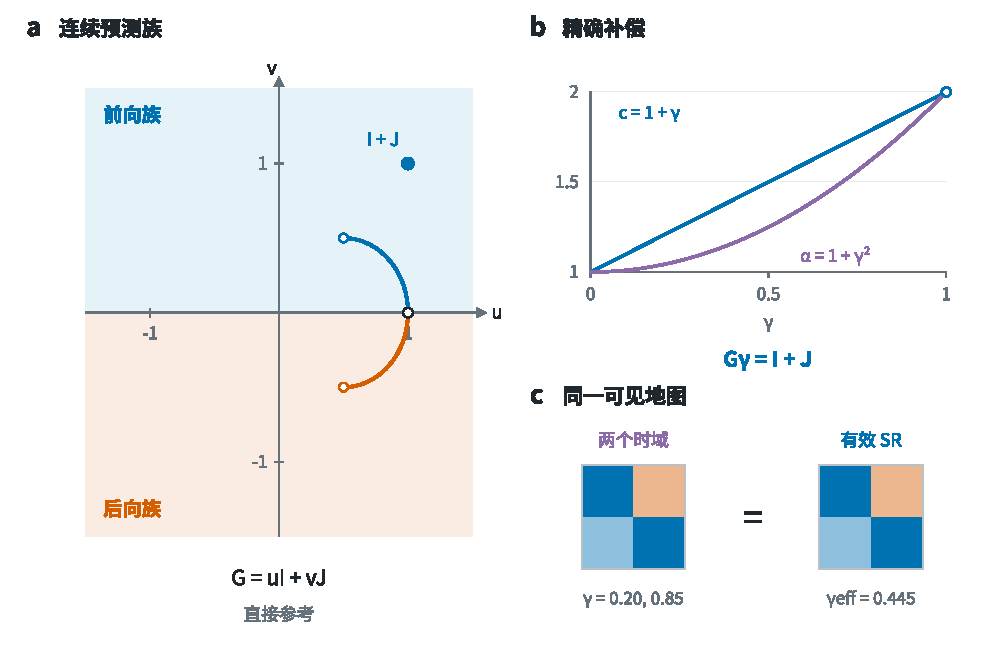
\includegraphics[width=\linewidth,height=0.64\textheight,keepaspectratio]{figures/pdf/fig02_families_zh.pdf}
\vspace{3pt}
\begin{minipage}{\linewidth}
\fontsize{9.2}{11.7}\selectfont
\setlength{\parskip}{3pt}

\textbf{图 2. 连续预测族区分共同性质与唯一参数值。}
\textbf{a，}四分之一旋转任务平面上，\(J=\left(\begin{smallmatrix}0&-1\\1&0\end{smallmatrix}\right)\)，已知直接参考使作用
\(G=uI+vJ\) 可见。对于 \(G_+=cI+\alpha J(I-\gamma J)^{-1}\)，当
\(c\in\mathbb R\)、\(\alpha\geq0\)、\(0\leq\gamma<1\)
遍历全部允许值时，前向预测族覆盖 \(v\geq0\)，后向预测族覆盖
\(v\leq0\)。阴影矩形是无界半平面的一个有限视窗。弧线显示约束更强、整体增益为一的完整
SR \(M_\gamma(\pm J)\)；空心端点表示 \(\gamma\to1\)
的极限。\textbf{b，}在当前状态系数可自由变化的这一模型族内，对每个允许折扣，\(c=1+\gamma\)、\(\alpha=1+\gamma^2\)
都给出同一个 \(I+J\)，对应 a
中的标记点。这些解释的方向共同为前向，折扣却可连续变化。该标记算子位于正增益完整
SR 族之外，因为后者在 \(\gamma<1\) 时满足
\(v/u=\gamma<1\)。\textbf{c，}共享同一特征映射、折扣分别为 \(0.20\) 与
\(0.85\) 的等权完整 SR 混合，与一个正增益缩放的单折扣完整 SR
具有完全相同的二维算子。有效折扣约为
\(0.445\)，有效增益记录在源数据中。两矩阵的系数相同，蓝、橙分别表示正、负值。这些确定性恒等式联系了性质辨识、参数补偿与多尺度等价。完整预测族结论见补充定理
T06、T16。

\end{minipage}
\end{figure}

\Needspace{6\baselineskip}
\subsubsection{3.4
互反任务让已学习条件提供新的方向约束}\label{ux4e92ux53cdux4efbux52a1ux8ba9ux5df2ux5b66ux4e60ux6761ux4ef6ux63d0ux4f9bux65b0ux7684ux65b9ux5411ux7ea6ux675f}

直接参考为前面的半平面结果提供了基础。现在回到参考本身已经学习的情形。我们让两个条件共享基础神经映射，同时改变它们的转移组织，询问这种实验约束能够增加什么信息。以下先考察完整
SR，再扩展到非负混合及已证明的额外当前成分。

\par
\noindent\begin{minipage}{\linewidth}

仍然使用四分之一旋转平面。由 \(J^2=-I\)，完整 SR 可以写为

\[
M_\gamma(J)=\frac{I+\gamma J}{1+\gamma^2}.
\]

\end{minipage}\par

这表示一个正缩放和角度为 \(\arctan\gamma\) 的旋转。同图两个前向 SR
的相对角度是
\(\arctan\gamma-\arctan\eta\)，因而会随目标与参考的时域关系改变符号。

\par
\noindent\begin{minipage}{\linewidth}

现在让目标任务在共同平面上作用为 \(J\)，参考任务作用为
\(-J\)。两个条件仍然各自向前预测，目标折扣为 \(\gamma\)，参考折扣为
\(\eta\)。从参考到目标的相对作用为

\[
T=aM_\gamma(J)M_\eta(-J)^{-1}.
\]

\end{minipage}\par

\par
\noindent\begin{minipage}{\linewidth}

目标具有正向角度，参考具有反向角度。取两者的相对关系后，角度相加：

\[
\phi=\arctan\gamma+\arctan\eta.
\]

\end{minipage}\par

只要至少一个折扣非零，这个角度就为正。两个条件都后向时，得到相反符号。我们固定目标、参考的顺序来解释符号；交换比较顺序，相对角也相应反号。

这一方向保证还可以推广到一般实压缩任务对比块。将其记为
\(A\)，两个实验条件在共同坐标中分别实施 \(A\) 与
\(A^\top\)，并保持正增益和共同神经映射。用任务的反对称部分
\(K=(A-A^\top)/2\) 表示带方向的作用，在 \(K\neq0\)
且至少一个折扣非零时，两个完整前向 SR 满足
\(\langle T,K\rangle_F>0\)，两个后向 SR
满足负号。这个结论允许非正规任务，也允许两个条件具有不同时域（补充材料
T08）。非负额外当前项的扩展范围在结果 4 中说明。

\par
\noindent\begin{minipage}{\linewidth}

实验实现还可以进一步简化。我们不必要求两张完整转移图处处反向，只需让用于分析的状态关系具有互反作用。考虑八状态环：第一种任务每次前进一个状态，第二种任务每次前进三个状态。它们的完整转移矩阵是
\(P\) 与
\(P^3\)。沿一对预定对比轴，八个状态的相位依次重复四个方向，因此前进一步相当于旋转
\(90^\circ\)，前进三步相当于旋转 \(270^\circ\)，也就是反向
\(90^\circ\)。令 \(C\) 提取这两条对比，便有

\[
CP=JC,\qquad CP^3=-JC.
\]

\end{minipage}\par

两任务都保持这个分析空间，使其中的作用能够独立描述。这称为共同约化子空间（图
3；补充材料
T11）。它提供一种利用相同刺激、不同序列组织获得互反信息的方式。多序列任务已经为研究情境相关的过去与未来表征提供了实验背景
{[}8{]}；共同子空间分析进一步指出，哪些明确的任务关系可以承载这里的识别保证。

\Needspace{6\baselineskip}
\subsubsection{3.5
允许方向切换后，哪些观测仍具有排他性}\label{ux5141ux8bb8ux65b9ux5411ux5207ux6362ux540eux54eaux4e9bux89c2ux6d4bux4ecdux5177ux6709ux6392ux4ed6ux6027}

两个实验条件可以改变传播结构，也可能改变参与者使用的机制。为此，我们将候选集合扩展为四种组合：目标与参考都前向（FF），都后向（BB），目标前向而参考后向（FB），以及目标后向而参考前向（BF）。前、后都相对于各条件自己的任务方向定义。

在上述 \(J,-J\) 任务中，两条件分别使用完整 SR，折扣遍历 \([0,g]\)，其中
\(g<1\)，整体正增益自由变化。令
\(h=\arctan g\)。计算全部参数产生的相对角度，得到精确范围：

\begin{longtable}[]{@{}ll@{}}
\toprule\noalign{}
两条件的机制 & 全部相对角度 \\
\midrule\noalign{}
\endhead
\bottomrule\noalign{}
\endlastfoot
FF & \([0,2h]\) \\
BB & \([-2h,0]\) \\
FB 或 BF & \([-h,h]\) \\
\end{longtable}

这张表把每个机制名称转成了完整经验预测（图 3；补充材料
T13）。在允许折扣小于一的整体范围内，\(30^\circ\) 可以由两个前向角度
\(15^\circ+15^\circ\) 产生，也可以由方向切换的 \(40^\circ-10^\circ\)
产生。配合合法的正增益，两种解释可以给出同一个相对算子。若只比较 FF 与
BB，就会遗漏后一种相容机制。

但这种扩展也留下明确的排他区域。由于每个完整 SR 的角度小于
\(45^\circ\)，一个前向、一个后向的组合，其相对角度限于
\((-45^\circ,45^\circ)\)。严格超过 \(45^\circ\)
的正角度，能够排除这两种切换解释和
BB；负外侧区域对应共同后向。对于有共同上限 \(g<1\)
的任务，边界相应缩小为
\(\pm h\)。采用严格越过边界的规则，也给有限误差下的判断留下清楚的几何对象。

连续族的意义在这里尤其直观。不同机制并不需要在每一处都分开，当前观测落在哪一部分才决定能说什么。交叠区保留多个解释，外侧区支持一个共同性质。这样的区分由完整参数范围得出，可以直接用于指导实验和误差分析。

进一步允许一个条件混合多个前向与后向完整
SR，只要各成分共享神经映射、权重非负，额外当前项也非负，总作用非零时仍可写成
\(uI+vJ\)，且
\(u>0\)、\(|v|\leq gu\)。因此同样的角度范围可以按各条件的净方向组织。正外侧区域要求两个条件都净前向；负外侧区域要求两个条件都净后向（补充材料
T14）。这里可识别的性质允许反向成分存在，它确定的是全部成分合成后的方向。多尺度组成继续保留在相容集合中，而方向的共同约束已经得到加强。

\begin{figure}[!htbp]
\centering
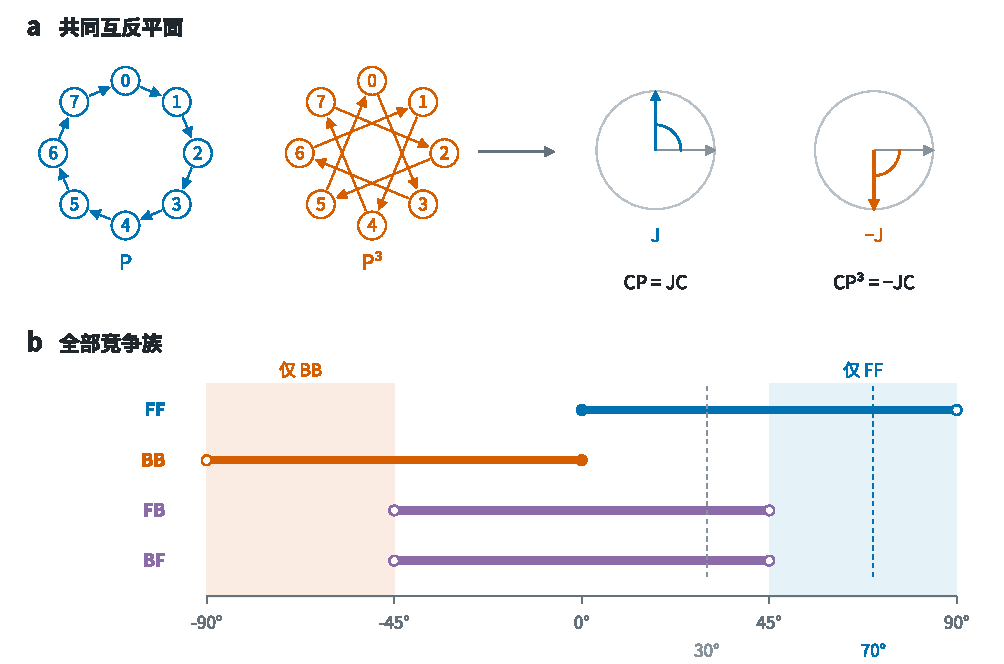
\includegraphics[width=\linewidth,height=0.64\textheight,keepaspectratio]{figures/pdf/fig03_reciprocity_zh.pdf}
\vspace{3pt}
\begin{minipage}{\linewidth}
\fontsize{9.2}{11.7}\selectfont
\setlength{\parskip}{3pt}

\textbf{图 3. 互反任务产生能够排除条件间方向切换的区域。}
\textbf{a，}同一带标签八状态环的一步和三步转移为 \(P\) 与
\(P^3\)。预定正交状态对比 \(C\) 满足
\(CP=JC\)、\(CP^3=-JC\)，因此两完整转移在共同约化平面上提供相反的四分之一旋转作用。该平面由任务定义，两完整矩阵无需互为转置。\textbf{b，}固定目标任务为
\(J\)、参考任务为 \(-J\)，假设共同特征映射、正整体增益及折扣位于
\([0,1)\) 的纯完整 SR。FF 的相对角度范围为 \([0,90^\circ)\)，BB 为
\((-90^\circ,0]\)，FB 与 BF 为
\((-45^\circ,45^\circ)\)；字母依次表示目标、参考条件的前向或后向编码。空心端点表示不能达到的极限。\(30^\circ\)
灰线同时穿过 FF 与方向切换族，\(70^\circ\) 蓝线只穿过
FF。阴影标出用于稳健排除切换的严格外侧区域。若事先规定共同折扣上界
\(g<1\)，相应界限改为 \(\arctan g\) 与
\(2\arctan g\)，并包含对应闭端点。共享同一特征映射的非负完整 SR
混合保留相应净方向结论。一般条件见补充定理 T08–T09、T11–T14。

\end{minipage}
\end{figure}

\Needspace{6\baselineskip}
\subsubsection{3.6
任务相容读出保留方向所需的信息}\label{ux4efbux52a1ux76f8ux5bb9ux8bfbux51faux4fddux7559ux65b9ux5411ux6240ux9700ux7684ux4fe1ux606f}

上述结果说明了哪些作用关系有用。实际测量接下来需要回答，如何从许多神经通道中保留这些关系。恢复任意完整算子要求参考覆盖所有需要恢复的状态方向；如果科学问题只涉及某个作用的符号或角度，所需信息可以更少（补充材料
T10）。

我们先由任务结构提取共同平面，再用训练资料选择一个模板，并在正式比较前冻结它。读出将这个平面内的状态模式转成两个数。关键是让读出与任务作用相容：先施加任务作用、再读出，和先读出、再施加相应的二维作用，得到同样的关系。

\par
\noindent\begin{minipage}{\linewidth}

记这个线性读出为 \(z\)，相容性写为

\[
z\{(uI+vJ)X\}=(uI+vJ)z(X).
\]

\end{minipage}\par

一个具体构造是，将模式分别与训练模板及该模板经 \(J\)
旋转后的版本作内积。两个模板组成一对方向相差 \(90^\circ\)
的比较轴，因此保留了候选作用中的缩放与旋转关系。构造的完整公式及其交换恒等式见方法和补充材料
T12。

\par
\noindent\begin{minipage}{\linewidth}

令正式总体参考的读出为 \(b\)，目标为 \(y\)。如果原始模式满足共同关系
\(T=uI+vJ\)，读出后仍有

\[
y=(uI+vJ)b.
\]

\end{minipage}\par

\par
\noindent\begin{minipage}{\linewidth}

两向量形成的有向面积满足

\[
\det[b,y]=v\|b\|^2.
\]

\end{minipage}\par

只要真实参考投影 \(b\) 非零，面积的符号就保留了 \(v\) 的符号。再与点积
\(b^\top y=u\|b\|^2\)
合用，就能读取相对角度。于是，一对任务相容坐标可以保留方向性质，完整参考满秩成为一种更强目标所需的条件（图
4）。

这一读出围绕科学问题选择信息。训练模板不必等于真实参考，但正式参考必须在所选比较轴上留下非零信号。更多模板可以提高可见性或检查共同作用，所有模板则应保留在同一个重复单位中处理。对于在整个任务平面上已经相等的机制，增加同平面的模板会继续得到相同预测；区分它们需要另一个传播关系。

还可以在比较候选模型时，保留所有候选实际使用的共同预测空间。与模型间差异无关的方向，无需占据同样的误差预算。共同任务平面规定实验作用，相容读出保留这个作用，共同预测空间集中候选比较的有关部分。它们共同使信息需求与所要回答的问题对应起来。

\Needspace{6\baselineskip}
\subsubsection{3.7
联合误差将相容集合用于有限测量}\label{ux8054ux5408ux8befux5deeux5c06ux76f8ux5bb9ux96c6ux5408ux7528ux4e8eux6709ux9650ux6d4bux91cf}

到目前为止，我们讨论的是精确关系。有限测量中，参考和目标都围绕其总体模式变化，同一个重复单元内的误差还可能相关。判断方向时，我们需要把这些变化带入同一个相容集合。

\par
\noindent\begin{minipage}{\linewidth}

设正式资料由重复配对 \((b_i,y_i)\) 组成。对于一个候选作用
\(T_\theta\)，它预测目标均值等于参考均值经该作用变换后的结果。因此可以考察残差

\[
r_i(\theta)=y_i-T_\theta b_i.
\]

\end{minipage}\par

若候选关系正确，残差的总体均值应为零。残差协方差同时包含目标误差、参考误差和二者的配对相关。参考若变化较大，与它相乘的候选作用也会相应改变不确定性。联合处理保留了这一依赖关系。

给定独立训练后冻结的任务、模板和候选空间，在真正独立同分布的高斯配对单元、正定残差协方差以及重复数大于残差维数的条件下，我们反演
Hotelling 均值检验，保留全部与数据相容的连续候选。记保留集合为
\(\widehat{\mathcal C}_\alpha\)。当真实机制属于预定候选空间时，真实候选被保留的概率为
\(1-\alpha\)（方法；补充材料 T26）。

\par
\noindent\begin{minipage}{\linewidth}

性质声明继续使用同一条原则：保留集合非空，而且其中所有解释对目标性质一致，才作出该性质声明。若真实候选仍被保留，这样的共同性质必然与它一致。因此

\[
\Pr\{\text{作出性质声明且声明错误}\}\leq\alpha.
\]

\end{minipage}\par

这个保证直接连接连续模型族与科学结论。它控制整个判断程序作出错误声明的概率；已经作出声明之后的条件错误率是另一个统计目标。不同方向标签即使恰好给出同一个算子，也都保留在候选空间中，因而精确别名会自然表现为无法作出唯一方向声明。

同一套分析能够给出几种有明确意义的结果。所有相容候选共同前向时，声明前向性质；仍有相反方向时，保留方向歧义；没有候选相容时，检查预定机制与观测关系；参考没有可见投影或重复结构不足时，报告这一信息缺口。区分这些结果，使一个无法判断的实验仍能指出下一步需要增加什么。

误差控制也不要求两个连续族在全局处处相隔。若族的某些边界相交，全局最小距离可以为零，而当前观测仍可远离所有相反性质。我们的分离结果将这种局部判断写成误差邻域与候选距离的条件（补充材料
T25）。在实际应用中，窗口、模板与任务选择由独立训练确定，重复单位按照真实采集结构定义；这些条件在第六部分的真实校准中逐一对应。

这样，连续族给出要保留的解释，实验提供跨条件约束，任务相容读出保留性质相关的作用，联合误差决定有限数据可以排除哪些候选。方向与时域组成已经具有不同的识别地位。接下来，我们考察改变模型或测量前提时，这些保证如何随之变化，再进一步寻找能够恢复时间权重的信息。

\begin{figure}[!htbp]
\centering
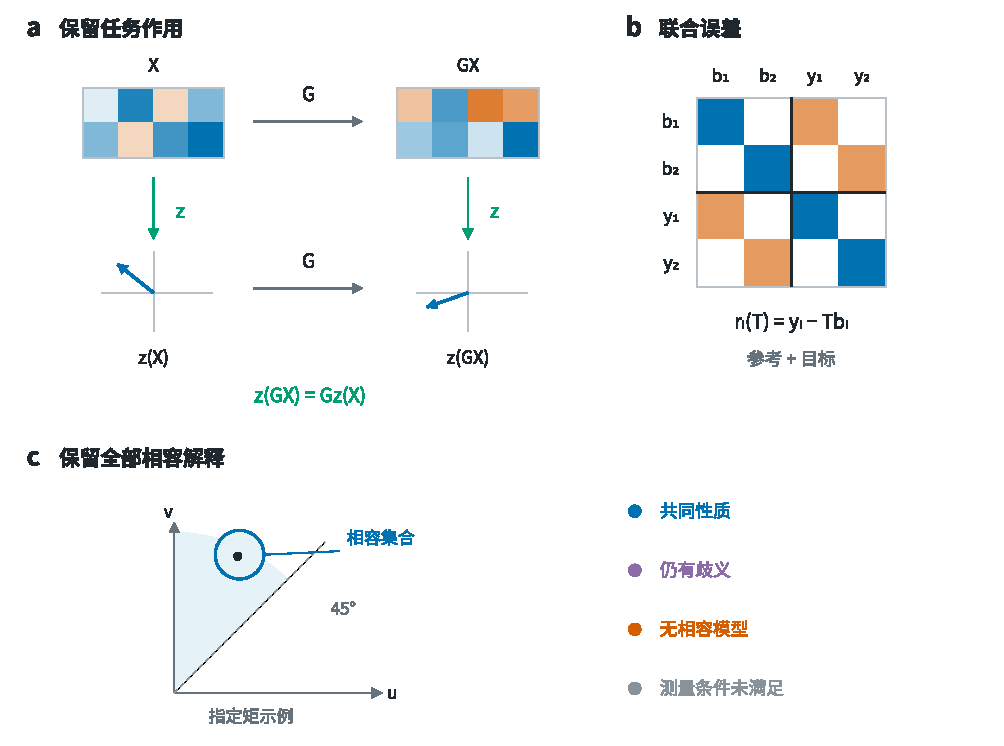
\includegraphics[width=\linewidth,height=0.64\textheight,keepaspectratio]{figures/pdf/fig04_measurement_zh.pdf}
\vspace{3pt}
\begin{minipage}{\linewidth}
\fontsize{9.2}{11.7}\selectfont
\setlength{\parskip}{3pt}

\textbf{图 4. 任务相容读出将机制关系带入低维统计问题。}
\textbf{a，}冻结模板 \(R\) 定义
\(z(X)=(\langle R,X\rangle_F,\langle JR,X\rangle_F)^\top/\|R\|_F\)。对于
\(G=uI+vJ\)，读出与任务作用可交换，即
\(z(GX)=Gz(X)\)。图中矩阵与坐标向量使用指定数值输入及
\(G=0.5I+0.8J\)。真实参考投影 \(b\) 非零时，有向面积满足
\(\det(b,Gb)=v\|b\|^2\)。\textbf{b，}参考与目标的变异通过
\(r_i(T)=y_i-Tb_i\) 共同进入推断。图示联合协方差的对角块为
\(0.04I_2\)，交叉块为
\(-0.025I_2\)；蓝、橙表示正、负元素。\textbf{c，}解析示例取
\(\bar b=(1,0)^\top\)、\(\bar y=1.2(\cos65^\circ,\sin65^\circ)^\top\)、\(n=24\)、\(\alpha=0.05\)。在
\(T=uI+vJ\) 上反演候选特定的二维残差检验，得到全部位于 \(v=u\)
上方的相容集合；在图 3 的四族实验中，该集合处于 FF
区域。此图由指定充分统计量构造。科学结论取决于完整保留集合：共同性质、尚存竞争解释，或具有额外约束的模型族整体不能相容。测量资格由参考可见性与采集设计评价。名义错误控制要求独立训练和真正独立同分布高斯配对检验单元。补充定理
T10、T12、T25–T28 区分了残差反演、联合均值覆盖与测量资格。

\end{minipage}
\end{figure}

\Needspace{7\baselineskip}
\subsection{4.
保证的边界来自哪些模型与测量条件}\label{ux4fddux8bc1ux7684ux8fb9ux754cux6765ux81eaux54eaux4e9bux6a21ux578bux4e0eux6d4bux91cfux6761ux4ef6}

到这里，方向判断已经有了一个明确含义：在规定的任务、参考与候选族中，留下来的解释是否共同具有前向或后向性质。这个问题之所以可以回答，是因为实验关系和模型约束共同排除了一部分可能性。理解这些约束怎样起作用，也就能理解保证的范围。下面的几个例子分别改变任务、权重和记录过程，观察原来的结论如何随之变化。

\Needspace{6\baselineskip}
\subsubsection{4.1
方向首先需要一个共同的任务坐标}\label{ux65b9ux5411ux9996ux5148ux9700ux8981ux4e00ux4e2aux5171ux540cux7684ux4efbux52a1ux5750ux6807}

“向前”总是相对于某条已知的状态关系而言。假如参与者实际学习到的转移完全自由，那么前向使用一个内部转移，与后向使用它的时间反转，可以生成同样的预测。形式上，如果允许的内部转移集合在时间反转下封闭，前向族与后向族的观测范围就完全相同（补充命题
T05）。这时缺少的是方向的参照，而不仅是对神经模式的精确估计。

实验中的转移操控、序列记忆测试和行为选择可以为这个参照提供独立依据。它们所约束的是参与者使用了哪些状态关系。与此相配，跨条件比较还需要共同的神经映射：相同状态成分应当通过同一组基础关系进入记录。固定电极和刺激集合有助于实验控制，共同映射本身则由这些控制及参考测量共同支持。模型中的任务与映射因此都有明确的经验角色。

\Needspace{6\baselineskip}
\subsubsection{4.2
当前反应的自由度会改变互反结论}\label{ux5f53ux524dux53cdux5e94ux7684ux81eaux7531ux5ea6ux4f1aux6539ux53d8ux4e92ux53cdux7ed3ux8bba}

\par
\noindent\begin{minipage}{\linewidth}

完整 SR
把当前项与预测项按同一个规则绑定。第三部分的互反方向保证，以及完整 SR
加非负当前成分的若干扩展，都利用了这种结构。若允许当前权重和预测增益独立变化，候选范围会扩大到

\[
G_\sigma=cI+\alpha N_\gamma(\sigma J),
\qquad N_\gamma(A)=A(I-\gamma A)^{-1}.
\]

\end{minipage}\par

其中，\(\sigma=+1\) 与 \(-1\) 分别标记相对于任务的前向与后向作用。

在两个都已学习的条件中，这种扩大可以重新引入精确换向别名。取
\(\gamma=1/2\)、\(\alpha=5\)，一套前向解释的当前权重为
\(c=1\)，在两互反条件中分别产生 \(-I+4J\) 与 \(-I-4J\)。另一套后向解释取
\(c=3\)，产生 \(I-4J\) 与
\(I+4J\)；若其共同映射为原映射的相反数，两个条件的全部平面模式同时保持不变（补充反例
T07）。每套解释内部都有共同映射，两套解释的机制方向却相反。

这与直接参考下的方向半平面结果具有清楚的关系。直接参考将基础映射锚定下来；两个学习条件的比较则仍允许不同解释采用不同的共同映射。改变的正是可用信息。另一方面，完整
SR
加非负额外当前项保留了较强约束，其互反符号保证已延伸到二维块、任意维正规块与平方零块（补充命题
T09）。因此，当前成分如何进入模型，应当与折扣范围一起成为科学假设的一部分。

\Needspace{6\baselineskip}
\subsubsection{4.3
过去的信息也可能来自记录过程}\label{ux8fc7ux53bbux7684ux4fe1ux606fux4e5fux53efux80fdux6765ux81eaux8bb0ux5f55ux8fc7ux7a0b}

\par
\noindent\begin{minipage}{\linewidth}

还有一种后向模式与内部预测无关。设神经系统在每一时刻只编码当前状态，但记录中保留了先前响应：一次刺激的活动尚未消退，下一次刺激已经到来。给定当前状态，先前状态的条件分布由时间反转
\(P^*\) 描述。因此，这种历史残留的平均模式可以写成

\[
\mathbb E[Y_t\mid S_t]
=\sum_{\ell\geq0}h_\ell(P^*)^\ell B,
\]

\end{minipage}\par

其中 \(h_\ell\) 是记录对过去第 \(\ell\)
步响应的权重。若这些权重按等比衰减，就得到一个后瞻 SR 的形式（补充定理
T23）。同一个矩阵表达式，在这里描述的是记录的历史，而不是内部表征对过去的计算。

这一结果将两个时间尺度分开：任务传播以状态转移步数计，测量残留则以实际经过的时间计。改变呈现间隔、估计独立响应核和安排独立探测试次，都可以增加区分二者的信息。对于稳定且绝对可和的线性历史核，独立同分布的探测使过去状态的平均贡献与当前身份无关；去除共同状态成分后，这部分不再产生方向模式。这个条件要求过去与当前身份真正独立，不能仅凭“呈现顺序随机”来判断是否成立。互反任务也会反转测量历史的条件关系，因此历史控制与互反操控承担不同任务。

\Needspace{6\baselineskip}
\subsubsection{4.4
一个性质可以确定，模型仍有其他内容等待检验}\label{ux4e00ux4e2aux6027ux8d28ux53efux4ee5ux786eux5b9aux6a21ux578bux4ecdux6709ux5176ux4ed6ux5185ux5bb9ux7b49ux5f85ux68c0ux9a8c}

在单平面上，只要参考向量 \(b\neq0\)，任意目标向量 \(y\) 都可以唯一写为
\(y=(uI+vJ)b\)。当当前项和预测增益自由时，前后两族合在一起便能描述每一对这样的均值。\(v\)
的符号仍具有该族内的方向意义，但单凭这一对均值，整体模型已经没有剩余的适配约束（补充定理
T06）。

这说明应当区分两种任务：在一个模型族内部判断性质，以及检验这个模型族能否解释数据。增加独立模板可以检查同一作用是否在多个读出上成立；增加传播性质不同的任务块，则可以检查同一组参数是否同时解释这些关系。后者还提供了拆开单尺度与多尺度别名的机会，因为在一个平面上完全相同的算子，不会仅因重复测量得更精确而分开。

结构可辨也有精度层面的要求。参考很弱、预测成分接近零或传播形状近乎相关时，竞争解释可能离得很近。更多有效独立重复可以缩小误差，但具体判定仍取决于当前观测到竞争族的距离。两个族在别处相交，并不妨碍这份观测位于可判区域；同样，两个方向在理想条件下不同，也不保证每次测量都足够精确。连续族与联合误差将这两个问题分别写清楚（补充命题
T25–T28）。

\Needspace{7\baselineskip}
\subsection{5.
从方向性质走向折扣与时间权重}\label{ux4eceux65b9ux5411ux6027ux8d28ux8d70ux5411ux6298ux6263ux4e0eux65f6ux95f4ux6743ux91cd}

前面的结果留下了一个建设性问题：如果已经知道当前观测支持哪种方向，还需要什么，才能知道它预测多远，或者怎样结合不同未来距离？答案取决于我们希望获得多精细的解释。某些观测首先限制参数范围；另一些任务让不同折扣产生独立形状；有限记忆设计则使各个滞后分别可见。我们依次考虑这些情况。

\Needspace{6\baselineskip}
\subsubsection{5.1
方向区域已经包含部分定量信息}\label{ux65b9ux5411ux533aux57dfux5df2ux7ecfux5305ux542bux90e8ux5206ux5b9aux91cfux4fe1ux606f}

\par
\noindent\begin{minipage}{\linewidth}

在互反的四分之一旋转平面上，两个纯完整前向 SR 满足

\[
\phi=\arctan\gamma+\arctan\eta.
\]

\end{minipage}\par

\par
\noindent\begin{minipage}{\linewidth}

假设相对角度恰好为 \(70^\circ\)。由于两个折扣都小于一，每一项角度都小于
\(45^\circ\)；为了使它们相加达到 \(70^\circ\)，每一项又必须大于
\(25^\circ\)。因此

\[
\gamma>\tan25^\circ\simeq0.4663,
\qquad \eta>\tan25^\circ\simeq0.4663.
\]

\end{minipage}\par

这个推理不需要选择最佳拟合点。满足角度关系的两个折扣仍然构成一条连续曲线，但曲线上的每个点都排除了过短的时域（图
5a）。这些下界是尖锐的：让一个折扣趋近一，另一个就能逼近相应下界。补充定理
T15 给出一般角度和共同折扣上限下的完整参数集合。

在实际数据中，可以把联合相容集合投影到折扣轴，直接报告仍然允许的范围。若候选是多尺度混合，相同角度约束的是有效相位比；要进一步约束每个组成时域，就需要能够区分核形状的观测。因而部分识别既给出当前信息，也指出剩余问题在哪里。

\Needspace{6\baselineskip}
\subsubsection{5.2
三种传播形状决定何时能够唯一恢复参数}\label{ux4e09ux79cdux4f20ux64adux5f62ux72b6ux51b3ux5b9aux4f55ux65f6ux80fdux591fux552fux4e00ux6062ux590dux53c2ux6570}

\par
\noindent\begin{minipage}{\linewidth}

单平面中，折扣变化可以被当前权重和预测增益补偿。要使这种补偿失效，任务必须让不同传播步长在记录中留下独立形状。考虑指定方向分支、已知任务
\(P\) 与总体直接参考 \(B\) 下的模型

\[
Y=cB+\alpha P(I-\gamma P)^{-1}B,
\qquad c\in\mathbb R,\quad\alpha>0,\quad0\leq\gamma<1.
\]

\end{minipage}\par

\(B\) 是直接形状，\(PB\) 是传播一步后的形状，\(P^2B\)
是传播两步后的形状。我们证明，三个参数 \(c,\alpha,\gamma\)
具有全局结构唯一性，当且仅当这三个矩阵线性独立（补充定理
T17）。这里把每个矩阵展开为一个向量，再检查三个形状是否相互独立。

为什么正好是三个？比较两组参数所产生的观测，消去两个逆矩阵后，会得到
\(B\)、\(PB\) 与 \(P^2B\)
的一个线性组合。如果这三个形状独立，各项系数就只能分别为零，从而迫使参数相同。若它们相关，传播已经落在一个过小的空间，当前项与预测增益便可以吸收折扣的变化。完整证明给出两种情形的必要与充分方向。

这个条件把实验设计的目标变得具体。增加通道有时会使更多传播形状可见，但通道数本身不是这里的条件。一个少通道、却保留独立传播形状的参考，可以比一个高维但形状重复的参考包含更多参数信息。参数恢复需要的是这些形状及其稳定性。

\Needspace{6\baselineskip}
\subsubsection{5.3
两个不同平面怎样提供共同约束}\label{ux4e24ux4e2aux4e0dux540cux5e73ux9762ux600eux6837ux63d0ux4f9bux5171ux540cux7ea6ux675f}

两个旋转性质不同的任务平面给出一个直观实现。在四分之一旋转平面中，我们已经看到许多参数组都能产生
\(I+J\)。让同一组参数再解释另一个旋转角不同的平面，原先的补偿就多了一项要求：它必须同时维持第二个平面的结果。

\par
\noindent\begin{minipage}{\linewidth}

设两块任务作用为 \(A_j=a_jI+\beta_jJ\)，其中
\(a_j^2+\beta_j^2=1\)、\(\beta_j>0\)，且 \(a_1\neq a_2\)。在共享
\(c,\alpha,\gamma\) 时，两块的旋转系数为

\[
v_j=\frac{\alpha\beta_j}{1-2a_j\gamma+\gamma^2}.
\]

\end{minipage}\par

将 \(v_1/\beta_1\) 与 \(v_2/\beta_2\)
相除，共同预测增益消去；剩下的比值唯一确定合法范围内的折扣。随后恢复
\(\alpha\)，再由各平面的非旋转部分恢复 \(c\)（补充定理 T18；图
5b）。八状态循环的 \(90^\circ\) 与 \(45^\circ\)
两个平面就能实现这一结构。

第二个平面还带来一个额外机会：从两块分别计算的当前权重必须一致。这是一条可以失败的预测。因此增加信息不只使参数更容易估计，也使模型受到更多检验。共享参数是这项设计的关键；若每个平面各自选择全部参数，两者之间的共同约束就消失了。

\begin{figure}[!htbp]
\centering
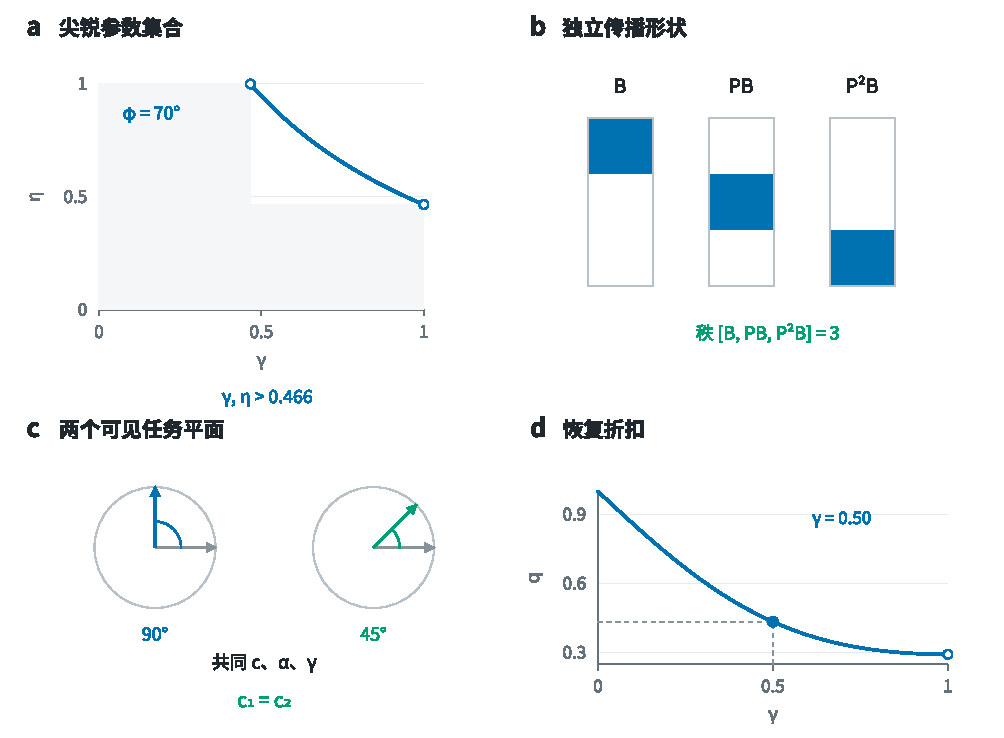
\includegraphics[width=\linewidth,height=0.64\textheight,keepaspectratio]{figures/pdf/fig05_quantitative_zh.pdf}
\vspace{3pt}
\begin{minipage}{\linewidth}
\fontsize{9.2}{11.7}\selectfont
\setlength{\parskip}{3pt}

\textbf{图 5. 额外传播信息将方向判断细化为参数约束。}
\textbf{a，}互反四分之一旋转实验中的两个纯完整前向 SR，若精确相对角为
\(70^\circ\)，则 \(\arctan\gamma+\arctan\eta=70^\circ\)。曲线是
\(0\leq\gamma,\eta<1\) 下的完整相容参数集合。两个折扣都超过尖锐下确界
\(\tan25^\circ\approx0.4663\)；空心端点表示极限，灰区被这一边缘界排除。\textbf{b，}对指定方向分支、已知任务
\(P\) 和直接参考 \(B\)，模型 \(Y=cB+\alpha P(I-\gamma P)^{-1}B\) 在
\(c\in\mathbb R\)、\(\alpha>0\)、\(0\leq\gamma<1\)
上参数唯一，当且仅当向量化后的三个矩阵 \(B,PB,P^2B\)
线性独立。图示约化例为 \(B=e_1\)、\(PB=e_2\)、\(P^2B=e_3\)，可嵌入图 6
的有限记忆任务，只使用一个已知参考列。\textbf{c，}同一八状态环提供可见的
\(90^\circ\) 与 \(45^\circ\) 旋转块，共同参数 \(c,\alpha,\gamma\)
必须同时解释两者。恢复参数后，两块给出的 \(c\)
还必须一致，留下额外模型检查。\textbf{d，}归一化旋转系数比为
\(q=1-\sqrt2\gamma/(1+\gamma^2)\)，在合法区间严格递减。标记点为
\(\gamma=0.5\)、\(q=0.4343146\)。令 \(t=(1-q)/\sqrt2\)，可由
\(\gamma=2t/(1+\sqrt{1-4t^2})\)
唯一反解。这些结构结果要求相应系数可见；有限数据精度取决于参考和系数的不确定性。证明见补充定理
T15、T17–T18。

\end{minipage}
\end{figure}

\Needspace{6\baselineskip}
\subsubsection{5.4
用有限记忆任务分开不同未来步长}\label{ux7528ux6709ux9650ux8bb0ux5fc6ux4efbux52a1ux5206ux5f00ux4e0dux540cux672aux6765ux6b65ux957f}

若问题进一步涉及整个时间权重形状，我们可以直接安排一项使不同滞后可分的任务。设每个状态由四位二进制数表示，例如
\(0101\)。每一步删除第一位，并随机追加一位，因此它会转到 \(1010\) 或
\(1011\)，两者概率各为一半。经过四步，初始四位已经全部被替换。

全部十六个状态构成一个二元 de Bruijn 转移图
{[}27{]}。对记录作四个预定对比，分别比较某一位为零与为一的状态，任务的作用就成为一个向下移位矩阵
\(N\)，其中 \(N_{i+1,i}=1\)，其余元素为零。它满足
\(N^4=0\)：四步后，起初的信息在这个对比空间中完全消失。整个随机任务仍持续运行（图
6a；补充命题 T19）。

\par
\noindent\begin{minipage}{\linewidth}

我们把不同预测步长的权重序列称为时间核。在循环任务中，绕行一圈后的较远滞后可能回到同一种传播形状，因此有限基上的系数会合并更远尾部的贡献。有限记忆块将这个关系明确分开：达到记忆长度后的初始信息在所用对比上消失，任意时间核在可见块上变成

\[
f(N)=w_0I+w_1N+w_2N^2+w_3N^3.
\]

\end{minipage}\par

现在，当前、一步、两步与三步的贡献分别位于不同矩阵位置。一个时间权重不再能够仅靠改变另一个权重，就在整个可见块上保持原来的作用。合格直接参考与相应算子方向的可见性，使这些系数可以逐项读出。

\Needspace{6\baselineskip}
\subsubsection{5.5
时间核可以直接检验单尺度与多尺度关系}\label{ux65f6ux95f4ux6838ux53efux4ee5ux76f4ux63a5ux68c0ux9a8cux5355ux5c3aux5ea6ux4e0eux591aux5c3aux5ea6ux5173ux7cfb}

\par
\noindent\begin{minipage}{\linewidth}

单一完整 SR 对各步采用同一个几何规则，因而前三个正滞后权重必须满足

\[
w_2^2=w_1w_3.
\]

\end{minipage}\par

\par
\noindent\begin{minipage}{\linewidth}

这个等式消去了整体尺度，也将当前项留在一旁。对于各尺度共享同一神经映射的同方向非负混合，\(w_h=\int\gamma^h\mu(d\gamma)\)，则有

\[
w_2^2\leq w_1w_3.
\]

\end{minipage}\par

\par
\noindent\begin{minipage}{\linewidth}

当 \(w_1>0\) 时，两边差异还具有直接含义：

\[
\frac{w_1w_3-w_2^2}{w_1^2}
=\operatorname{Var}_{\nu}(\gamma),
\qquad\nu(d\gamma)=\frac{\gamma\mu(d\gamma)}{w_1}.
\]

\end{minipage}\par

它是以正滞后贡献重新加权后的折扣方差。不同的有效预测时域越分散，这个量就越大（图
6c；补充定理
T20）。与单平面的有效折扣相比，有限记忆块因此提供了直接检验时间权重形状的机会。

可识别的范围仍由任务记忆长度决定。四位任务给出前三个正滞后；更长的二元记忆任务可以延长这一范围。零折扣成分不贡献正滞后，因而保留在这些观测的不可见部分。对无限远未来的推断，则还需要核的结构假设或更多可见滞后。

\Needspace{6\baselineskip}
\subsubsection{5.6
已学习参考中的目标核仍可被分离}\label{ux5df2ux5b66ux4e60ux53c2ux8003ux4e2dux7684ux76eeux6807ux6838ux4ecdux53efux88abux5206ux79bb}

前面的时间核读出采用直接参考。现在回到第二部分的问题：如果参考本身已经学习，是否仍有办法知道目标的权重？在有限记忆设计中，反向参考的三角结构给出一个出口。

\par
\noindent\begin{minipage}{\linewidth}

设目标为 \(f(N)\)，参考为未知 \(q(N^\top)\)，且其当前系数
\(q_0\neq0\)。两条件的相对作用为

\[
T=af(N)q(N^\top)^{-1}.
\]

\end{minipage}\par

\par
\noindent\begin{minipage}{\linewidth}

因为 \(N^\top\)
向上移位，它作用于第一基向量时为零。因此参考逆在这一向量上只产生
\(1/q_0\) 的缩放。相对算子的第一列便满足

\[
T_{h+1,1}=\frac{af_h}{q_0}.
\]

\end{minipage}\par

换言之，参考会改变整体尺度，却在这一列中保留目标各滞后的比例。只要这些元素可见，就能恢复目标有限核的相对形状；按符号解释方向时取
\(a/q_0>0\)。对两个纯完整
SR，矩阵中进一步的关系还能分别确定目标和参考折扣（图 6d；补充定理
T21）。

学习参考因而有两面：在某些任务上，它使相反机制产生相同相对作用；在另一些任务上，已知结构让目标与参考分别留下可读出的痕迹。决定结果的是观测中保留了什么关系。

\begin{figure}[!htbp]
\centering
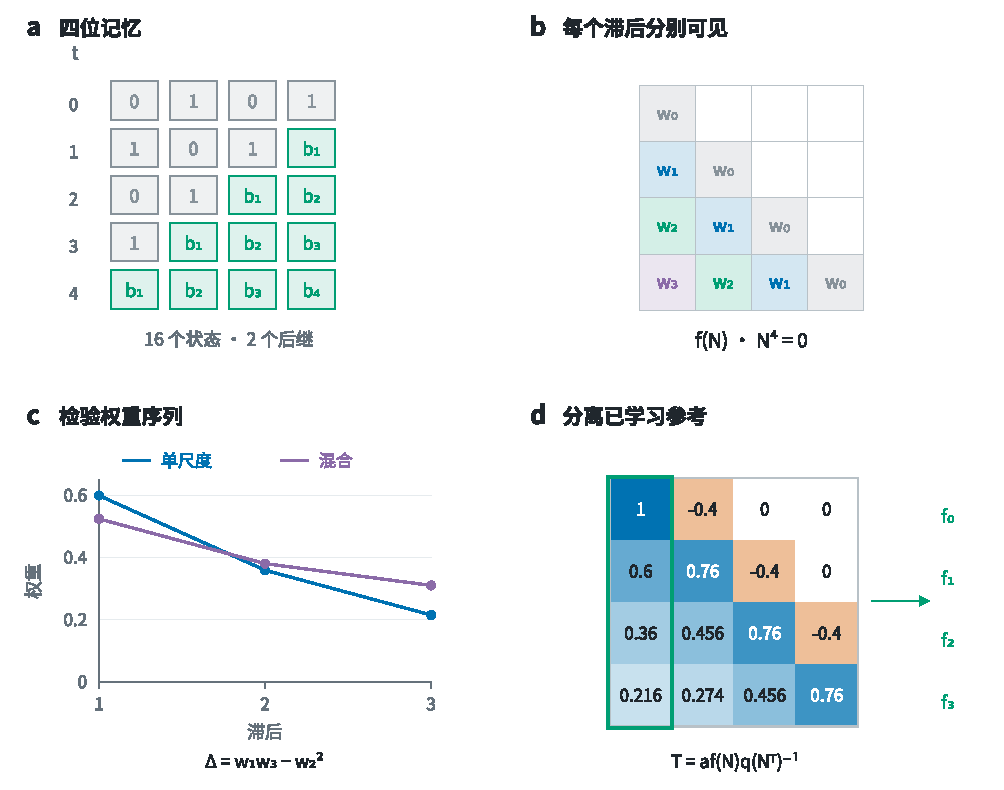
\includegraphics[width=\linewidth,height=0.64\textheight,keepaspectratio]{figures/pdf/fig06_kernels_zh.pdf}
\vspace{3pt}
\begin{minipage}{\linewidth}
\fontsize{9.2}{11.7}\selectfont
\setlength{\parskip}{3pt}

\textbf{图 6. 有限记忆任务使时间核分别可见。}
\textbf{a，}每个状态为四位二元字，每一步删除首位、追加独立等概率位
\(b_t\)。全部十六个字形成每状态有两条出边的双随机 de Bruijn
任务。图示路径说明初始四位如何被逐步替换。\textbf{b，}预定比特对比给出下移位块
\(N_{i+1,i}=1\)，满足 \(N^4=0\)。因此任意时间核在该块上成为
\(f(N)=w_0I+w_1N+w_2N^2+w_3N^3\)，不同正滞后占据不同副对角线。初始对比信息消失后，完整随机过程仍继续运行。\textbf{c，}折扣为
\(0.6\) 的单一完整 SR 具有权重 \((0.6,0.36,0.216)\)，且
\(\Delta=w_1w_3-w_2^2=0\)。共享特征映射、折扣为 \(0.2\) 与 \(0.85\)
的等权非负混合给出 \((0.525,0.38125,0.3110625)\) 和
\(\Delta=0.01795625\)。一般地，\(\Delta\geq0\)；当 \(w_1>0\)
时，\(\Delta/w_1^2\)
为按正滞后重新加权的折扣方差。有限可见权重仍不能确定零折扣质量与更晚滞后。\textbf{d，}参考已在反向任务学习时，\(T=af(N)q(N^\top)^{-1}\)
的第一列满足 \(T_{h+1,1}=af_h/q_0\)，其中
\(q_0\neq0\)。因此高亮首列保留目标核的共同尺度等价类。示例采用目标折扣
\(0.6\)、反向参考折扣 \(0.4\)、增益一；图中条目四舍五入，首列为
\((1,0.6,0.36,0.216)^\top\)。纯 SR
子族中，\(\gamma=T_{21}/T_{11}\)、\(\eta=-T_{12}/T_{11}\)
可恢复两个折扣。方向解释要求
\(a/q_0>0\)，并且相应算子条目可见。各面板均为确定性构造。一般结果见补充定理
T19–T21。

\end{minipage}
\end{figure}

\Needspace{6\baselineskip}
\subsubsection{5.7
净方向为零之后，仍有机制性质可以判断}\label{ux51c0ux65b9ux5411ux4e3aux96f6ux4e4bux540eux4ecdux6709ux673aux5236ux6027ux8d28ux53efux4ee5ux5224ux65ad}

方向统计为零时，我们也可以继续提出更细的问题。例如，一种机制用同一折扣形成前向与后向地图，再将两张地图等权混合；另一种机制先将转移关系对称化，再用正折扣形成
SR。对称学习规则与对称转移之间的关系已有模型研究
{[}10{]}。这两种构造都没有净方向，却不是同一计算。

在四阶有限记忆块上，两者的对角线预测不同。前后地图混合的主对角保持共同水平；对称化转移后的多步传播包含返回路径，会产生不同的对角结构。共享的当前项与正增益保留这一可检验区别（补充命题
T22）。因此，一个方向统计没有给出正负答案，并不意味着更丰富的观测也没有机制信息。

这些例子共同给出了一条增加解释分辨率的路径：先报告所有相容解释共同具有的性质，再确定仍被允许的参数范围，并通过独立传播信息进入点参数或时间核恢复。这是科学问题的递进；统计上，性质与参数可以同时从同一个联合相容集合导出。当研究目标确实要求完整算子时，满秩参考与有效误差界也提供相应恢复路线（Methods；补充定理
T24）。

\Needspace{7\baselineskip}
\subsection{6.
真实测量中哪些机制信息能够被保留和用于判断}\label{ux771fux5b9eux6d4bux91cfux4e2dux54eaux4e9bux673aux5236ux4fe1ux606fux80fdux591fux88abux4fddux7559ux548cux7528ux4e8eux5224ux65ad}

前面的结果给出了获得机制信息的条件。实际神经记录还需要完成另一件事：把这些条件落实到有噪声、会变化的测量中。我们使用公开的重复神经测量，分别检查参考能否预测后来的响应、哪些误差真正影响候选比较，以及冻结读出能否在已知作用下保留方向信息。已知变换提供了可核对的答案，真实记录则保留了状态结构、测量波动和跨记录变化。这几种校准围绕同一个问题展开：一次具体记录能够支持多精细的机制判断？

\Needspace{6\baselineskip}
\subsubsection{6.1
任务相关的参考可以预测后来的神经测量}\label{ux4efbux52a1ux76f8ux5173ux7684ux53c2ux8003ux53efux4ee5ux9884ux6d4bux540eux6765ux7684ux795eux7ecfux6d4bux91cf}

首先需要知道，参考中是否有能够保留到另一份测量的信息。我们分析 Turner
等人的视觉位置 EEG 定位资料
{[}18{]}，使用一名参与者的两次记录、每次记录的两个实际采集块。每块较早的事件用于估计参考，较晚的事件用于评价；估计器只在较早资料内部选择。状态平面由
40 个位置的第一对正弦与余弦对比预先定义。

在这个平面上，早窗参考估计相对零模式降低预测损失 14.72\%，晚窗降低
26.87\%；晚窗四个实际块均有改善，早窗则在其中两个块改善（图
7）。零模式是在移除所有状态共同活动后，不预测任何状态差异的基线。超过它，意味着参考估计保留了可以预测后来测量的状态信息。

这个收益发生在研究问题指定的平面中。晚窗完整矩阵的平均预测损失仍高于其完整矩阵零基线，而有用的任务平面已经能够被预测。因此，参考质量应当相对于所需性质评价：恢复所有状态方向与保留某个机制关系，具有不同的测量要求。这里报告的是对后来真实测量的预测损失；参考随时间改变及评价噪声共同参与这一损失。补充
fMRI 分析中，Ekman 资料的一名参与者 V1 情境相对零模式另有 19.60\%
的改善，其余情境的收益较小或选择零估计（补充材料 E3、E7）。

\Needspace{6\baselineskip}
\subsubsection{6.2
将误差比较放在候选机制能够改变的空间}\label{ux5c06ux8befux5deeux6bd4ux8f83ux653eux5728ux5019ux9009ux673aux5236ux80fdux591fux6539ux53d8ux7684ux7a7aux95f4}

神经模式包含的误差，并非全部都会改变模型之间的比较。若所有候选预测都位于共同空间中，目标在该空间以外的分量，会给每个候选增加相同的平方误差。将它分离出来，候选之间的平方误差差值和相应最近族判决保持不变。若所有候选的当前系数还允许在实数域自由重新拟合，与当前参考平行的共同成分也可以消去。

我们在 Kern 的 MEG 与 Turner 的 EEG 重复测量上计算了这一差别
{[}18,25{]}。两个来源各一名参与者，两个时间窗、三个预定状态空间、四个复用划分及每折
18 个已知方向变换，共形成 864
个方向计算条件。已知施加的算子确定了正确预测，因此可以将它与错误候选的距离同实际重复误差比较；通过表示已观察误差小于保证最近族判别所需的分离余量。用全部观测误差评价最近模型族的分离充分条件时，没有条件通过；将误差限制到共同预测空间后，二元与多类判断各有
6 个条件通过；再消去可重新拟合的当前项，通过数分别增至 80 与 77（图
7；补充材料 E9）。

在这 77
个多类条件中，与充分条件匹配的最近模型族规则全部唯一恢复了施加的可见方向。对相同条件使用训练后冻结参数的原规则，39
个保留正确方向，37 个退化为仅当前响应，1
个选择对称解释。这个对照说明，分离距离必须与实际采用的判决规则相连接：重新拟合目标的最近族规则，可以直接使用真实点到错误族的距离；冻结参数的预测器还需要计入正确族训练参数的迁移误差。

这一校准以已知变换和实际重复差构造误差，直接检验确定性充分条件。它揭示了可以保留哪些判别信息，以及哪些误差预算过于保守。对未知自然机制进行统计声明时，误差范围还需要由独立重复测量建立。

\Needspace{6\baselineskip}
\subsubsection{6.3
任务与读出设计增加了真实噪声中的可判断情境}\label{ux4efbux52a1ux4e0eux8bfbux51faux8bbeux8ba1ux589eux52a0ux4e86ux771fux5b9eux566aux58f0ux4e2dux7684ux53efux5224ux65adux60c5ux5883}

随后，我们在参考和目标都含测量误差的情况下，使用配对残差反演。Turner
第二次记录可以按每个位置的第几次出现组成 38
张完整状态图；前四张用于训练，其余 34 张交替组成 17
对参考与目标基础测量。训练资料确定状态顺序、通道变换、模板与任务相容读出，之后冻结。

对另一份完整基础测量施加已知 SR
算子，便可以检查这套读出是否保留了其方向。三个非重复后向条件在名义
\(\alpha=.05/54\) 下越过方向排除边界：原生位置环的
\(\gamma=.95\)，以及训练所得设计任务的 \(\gamma=.8\) 和 \(.95\)。54 对应
27
个测量或任务情境与两个模板版本。设计任务的两个条件使用了更新后的模板形状，展示了任务安排与读出选择可以增加可判断的情境；只差共同正比例尺度的读出版本给出相同判决，因而合并报告。

三个结果来自同一人的同一早窗及同一组 17
对重组状态图。校准改变的是完整测量，包括信号与噪声；参与者实际经历的仍是原定位任务。这里比较的是已知算子与重复基础响应的关系，相应的候选与参考设置也不同于两个已学习互反条件的四族比较。残差检验的概率保证要求真正独立同分布的高斯配对及合格的共同参考关系。当前状态图是按事件重组的，名义阈值因此描述给定这些条件时的结果；方法开发过程及事件依赖在补充材料
E4–E5 中单独记录。

\begin{figure}[!htbp]
\centering
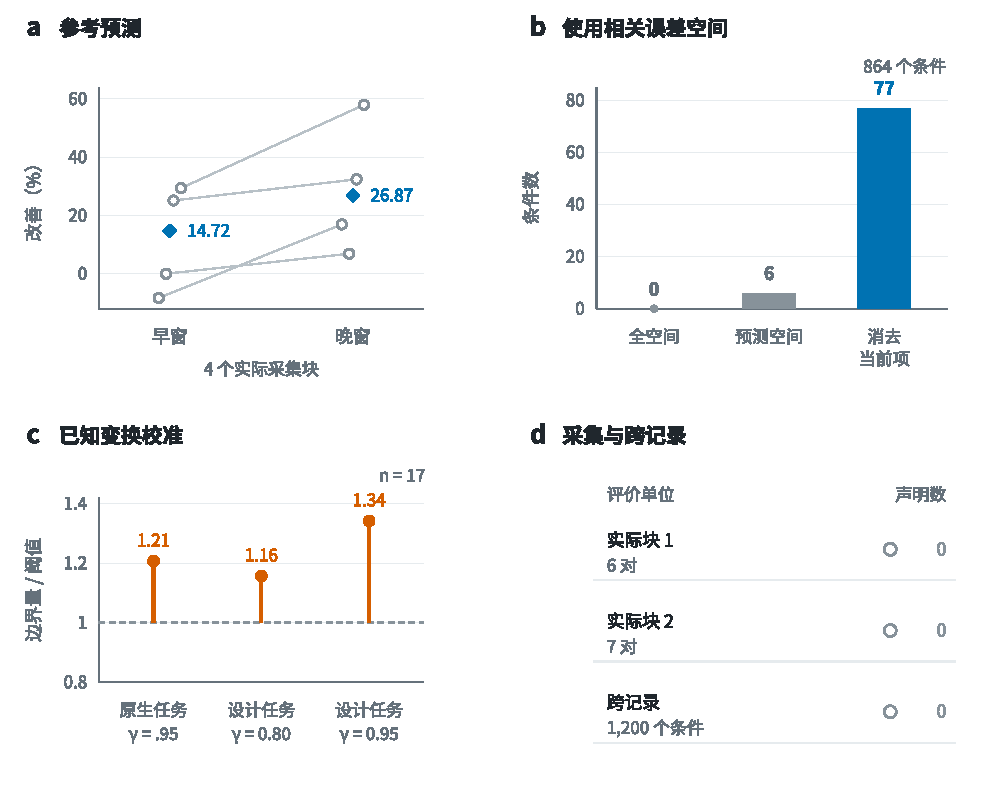
\includegraphics[width=\linewidth,height=0.64\textheight,keepaspectratio]{figures/pdf/fig07_calibration_zh.pdf}
\vspace{3pt}
\begin{minipage}{\linewidth}
\fontsize{9.2}{11.7}\selectfont
\setlength{\parskip}{3pt}

\textbf{图 7. 重复神经测量支持参考预测与有条件的机制校准。}
\textbf{a，}Turner EEG
一名参与者中，较早测量用于预测预定第一空间任务平面的较晚响应。空心点为两记录中的四个实际采集块，连线对应早窗（100–150
ms）与晚窗（200–250
ms）的同一块。菱形表示相对零模式预测器的改善，以一减去跨块平均预测损失之比计算，早窗为
14.72\%，晚窗为
26.87\%。菱形是平均损失之比，各空心点则是块级百分比。\textbf{b，}较早的已知变换校准汇集
Kern 与 Turner 各一人的 864
个折级方向计算条件。将误差预算置于全观测空间、共同预测空间、以及在该空间内消去可重新拟合的当前成分后，多类确定性充分条件通过数依次为
0、6、77。计数使用围绕已知变换参考的事后实际残差；与保证匹配的最近族规则在这
77 项中全部唯一恢复可见真方向。\textbf{c，}Turner
同一记录、同一早窗的三个非重复后向 SR
校准条件，其边界量与临界量之比超过一。原生任务 \(\gamma=.95\) 与设计任务
\(\gamma=.80,.95\) 共用同一组 17
对重组测量。已知算子施加于完整实际基础响应，同时变换其中的信号与噪声。名义水平为
\(.05/54\)，54 对应 27
个任务/测量情境与两个模板版本；独立同分布高斯配对单元是其明确采集要求。\textbf{d，}对设计任务后向
\(\gamma=.95\) 条件，分实际采集块分析分别保留 6、7
对，声明数均为零。冻结读出的跨记录评价，在 Kern 630 个与 Turner 570
个计算条件中也均未声明方向。这些采集检查明确了自然机制实验还需要的独立重复和参考稳定性。b
的保证来自已知真实误差下的确定性不等式，c–d
则采用上述统计校准；完整分析单位、预处理、选择过程与结果表见经验补充材料。

\end{minipage}
\end{figure}

\Needspace{6\baselineskip}
\subsubsection{6.4
实际采集层级决定哪些判断能够迁移}\label{ux5b9eux9645ux91c7ux96c6ux5c42ux7ea7ux51b3ux5b9aux54eaux4e9bux5224ux65adux80fdux591fux8fc1ux79fb}

完整状态图的重组与实际独立采集，是两种不同的重复。对设计任务中后向
\(\gamma=.95\) 的条件，分别限制在两个实际块内重构后，可用配对数为 6 和
7，两块均未越过相同校正门槛。样本量、均值与协方差在这项分析中一起改变，它具体指出了这一采集层级下的可判断范围。

进一步将来源记录训练的状态平面、白化、模板与读出全部固定，再应用于另一记录，Kern
的 630 个计算条件和 Turner 的 570
个计算条件均未作方向声明。跨记录参考变化与重复测量误差因而成为后续采集需要共同控制的对象。

这些真实测量将理论要求落实为可执行的步骤：任务相关参考可以具有预测收益；相容读出与恰当的误差空间可以保留可辨差异；概率声明还需要与真实采集单位相匹配。完整数据分支分别检验参考、传播形状、测量历史与分析约束，其方法、结果和来源见补充材料
E9–E11。沿这条路径，新的实验可以在采集时就提供独立的完整状态重复，并实际实施互反或有限记忆任务，使测量能力与机制问题在同一设计中相遇。

\FloatBarrier

\section{讨论}\label{ux8ba8ux8bba}

一份神经观测能够支持多精细的机制解释，取决于同它相容的解释之间还剩下什么差别。本文从预测地图出发，把这个问题逐步展开：距离几何可能保留状态关系而丢掉时间方向；参考校准可能揭示相对作用，却留下不同的机制来源；连续族中的某些性质可以确定，而具体折扣仍可变化。实验和读出的作用，就在于使与科学问题有关的差异留下来。第二个传播平面、有限记忆块和合格重复测量，分别让参数、时间核和有限样本声明获得进一步约束。

这些具体结果也把一个更一般的问题摆在面前：我们究竟凭什么从一次拟合，走向对心智一般规律的断言？图
8
将一般模型、特殊实例、实验观测与性质检验放在同一个关系中，作为以下讨论的纲领。

\begin{figure}[!htbp]
\centering
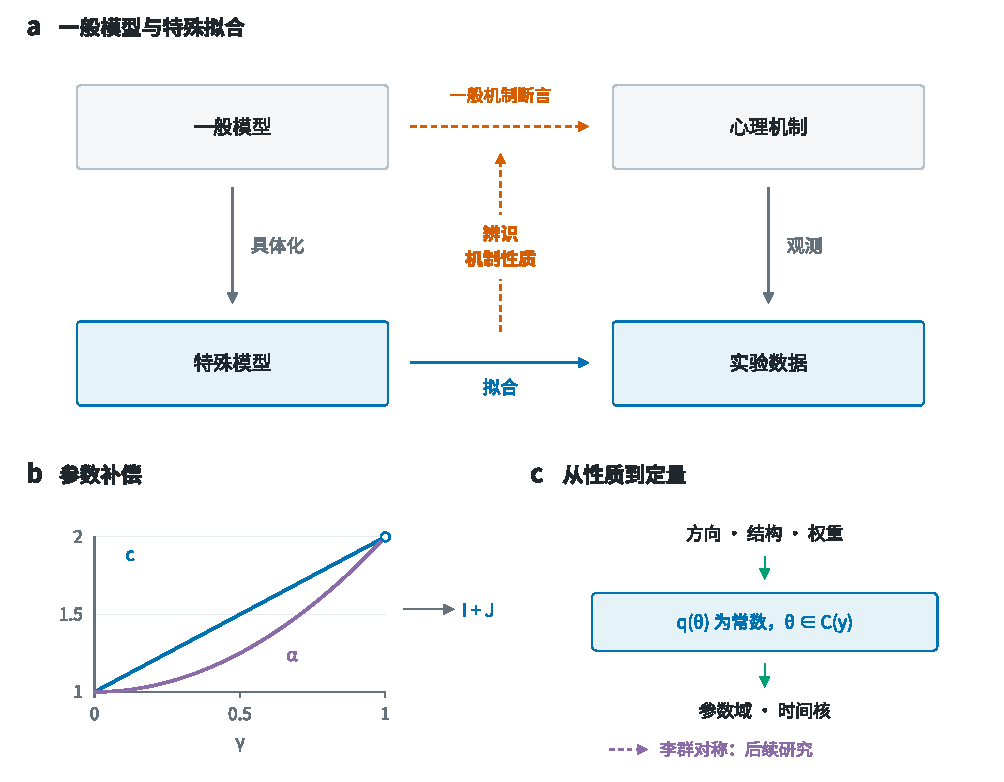
\includegraphics[width=\linewidth,height=0.64\textheight,keepaspectratio]{figures/pdf/fig08_programme_zh.pdf}
\vspace{3pt}
\begin{minipage}{\linewidth}
\fontsize{9.2}{11.7}\selectfont
\setlength{\parskip}{3pt}

\textbf{图 8. 一般模型、特殊拟合与性质辨识的研究纲领。}
\textbf{a，}作者的两层论证区分一般模型与心理机制，以及特定拟合模型与某次实验的观测数据。向下箭头分别表示参数和观测条件的具体化，以及对机制的实验测量。下层横向关系是拟合所检验的相符，上层横向关系是希望表达的一般机制断言；向上连接标出将两层联系起来所需的机制性质辨识。\textbf{b，}在当前状态系数可自由变化的直接参考四分之一旋转模型族中，当
\(c=1+\gamma\)、\(\alpha=1+\gamma^2\)
时，\(G_+=cI+\alpha J(I-\gamma J)^{-1}=I+J\) 在整个 \(0\leq\gamma<1\)
上成立。因此参数可以连续变化而观测完全相同，同时方向性质保持一致。空心端点表示不在域内的
\(\gamma=1\)
极限。\textbf{c，}时间方向、传播结构与时间权重都可以作为待检验的子性质。当某性质在全部相容解释
\(\mathcal C(y)\)
上恒定时，它就在规定模型类内得到辨识；额外独立实验约束可以进一步将相容集合细化为参数域或有限时间核。李群对称的虚线分支表示后续从指定对称性约束模型类的研究方向。图中保留作者关于一般模型与特殊模型的区分，参数补偿由本文
SR 结果提供解析实例，更广的研究纲领在 Discussion 中展开。

\end{minipage}
\end{figure}

\Needspace{7\baselineskip}
\subsection{一般模型、特殊模型与心理机制}\label{ux4e00ux822cux6a21ux578bux7279ux6b8aux6a21ux578bux4e0eux5fc3ux7406ux673aux5236}

我们常用计算模型拟合心理机制产生的数据。当计算模型拟合得好，我们便说心理机制服从计算模型。

这种做法是极危险的。从外表看，这是两个箱子，可以在有限的测试中表现出一样的行为。这是否可以说明两黑箱遵循相同的计算？即使排除掉有限测试集的偶然性——这个甚至不应该被轻易排除的限制——我们被放到一个先天优越的位置：两个模型
literally
表现完全相同，我们仍不具备充分的数学、逻辑学、哲学工具，确信它们机制是一致的。当然，两个系统可以产生相同反应，这个结果也绝非偶然；它们应该给我们一些保证，但这些保证我暂时还未进行研究。那上面那个该死的“拟合不等于解释”，究竟何以为然？其具体操作暴露了什么过当的声称？接下来，我们列出“拟合等于解释”的几宗罪。\footnote{拟合与理论支持的关系已有系统的方法学讨论
  {[}20{]}；参数恢复、模型恢复与定性行为检查也构成计算建模的重要实践
  {[}17{]}。这里的问题进一步指向，哪些可观察性质能够约束机制解释的范围。}

\textbf{拿特殊代表一般。}
心理学没有很多可复用的参数，即使很多有比较明确定义、而不依赖具体情境实验的变量，例如心理速度，也鲜被复用。这里的未复用有两种，一种鲜明，一种更隐蔽。鲜明的，即索性在新模型里，对这个被声称叫心理速度的变量直接拟合，不顾先前做过的研究，只是借一个变量名称而已。另一种更隐蔽：我确用了心理速度做参数，但心理速度参数还与另一个自由（将被拟合的）参数做了运算，而那个新自由参数在很大程度上只服务于此地，也就造成了原本是严格的“参数不可变”，变成先确定一个、而让另一个补偿的这种操作（Chen
et al., 2024）。\footnote{该例来自 Youguo Chen 及合作者关于视觉 Kappa
  效应的研究 {[}21,22{]}。2024 年研究固定经典模型的
  \(v_0=0.25^\circ/\mathrm{s}\)，以及低速模型的
  \(v_0=0.09^\circ/\mathrm{s}\)、\(t_0=1\,\mathrm{s}\)，同时估计其余参数。这一做法引出固定数值与固定可观察作用之间的区别；本文中的精确补偿由
  SR 恒等式具体给出（图 2、图 8b）。该研究的生产噪声参数 \(w_p\)
  作用于标准差，其作用须与均值增益区分。}
没有可复用的参数，模型被赋予的自由度就是极高的了。模型可以自由调整参数以适应数据，甚至发生严重的退化（图
8b）。

正由于心理学缺少可复用的参数，心理学对模型拟合成功这件事的理解又是极不准确的。如果用马尔可夫模型拟合了一个心理机制，人们便倾向于一个更简单的论断：“这个心理机制遵循马尔可夫过程。”或有的人可以更严谨一些：“马尔可夫过程可以描述这个心理过程。”然而，这些都是严重不准确的。一个依赖于精确参数拟合出来的现象，被升级为不依赖参数解释全过程。\footnote{这里讨论的是从某组参数、任务与读出中的相符，扩大到全过程或独特机制的解释范围。对已说明条件的一组数据，模型的描述性相符本身是明确而有意义的结论。图
  8a 的向上箭头标示需要进一步证据的范围扩展。} 看上面那张降维图（图
8a），实验者通常做的是下面，而希望表达上面，或被理解为上面。

那么如何？如果特殊不代表一般，心理学又如何发现心智的一般规律？上面讲了那么多，绝非说心理学没有价值。如果你也这么理解了，你也犯了如上科学家一样的错误。LOL。

有方法，那就是\textbf{如果做定性，就大大方方地做。}
什么是一般模型？一般模型并不必然等同于那个原始的大计算方程；那个带无数未知数的计算模型当然是一个方法。不过，由于参数往往未经过严格的定义域限制，我希望表达的其中一点是：参数定义域在什么范围仍可保证区分于其他模型的独特性，而不至于退化？更好的方法是，将其拆成几个更小的子性质，并通过数学方法发现该性质的充分、必要、充要条件，对数据进行检验和断言。

当然，对数据的定性研究并不必然需要留在定性，它也有方法为定量留出足够充分的门。其一，如果断言某一数据全称具备多种性质，我们可以期待用诸如反用李群对称的方法确定有限模型组。此外，如果指定了某个模型，甚至可以基于定性的稳固断言，确定参数域，并进行拟合（图
8c）。

\Needspace{7\baselineskip}
\subsection{以可检验性质组织模型与实验}\label{ux4ee5ux53efux68c0ux9a8cux6027ux8d28ux7ec4ux7ec7ux6a21ux578bux4e0eux5b9eux9a8c}

这份纲领在 SR
中有一个直接的实现。研究者先规定要判断的性质，再完整保留允许的方向、时域、当前成分与参考条件。相同观测对应的解释可能有很多，但它们未必在每个性质上都有分歧。直接参考的单平面例子保留方向，互反任务的外侧角区域进一步排除条件间切换，而有限记忆块把若干时间权重从有效折扣中分离出来。每一步都对应增加了什么约束，也对应能够说出什么结论。

这也给模型扩展提供了一个可比较的标准。加入自由参数之后，重要的问题是原来被识别的性质是否仍然在相容集合上保持一致。如果保持一致，这个性质就能跨越更宽的模型范围；如果不一致，新增自由度指出了原先结论所依赖的约束。实验可以据此安排新的观测。例如，单平面的时域混合促使我们测量独立传播形状，学习参考的别名促使我们研究互反关系与三角核结构。模型扩展因而可以直接指导下一项实验。

“定性之后走向定量”描述的是解释所需信息的关系。在统计实施中，方向、参数范围与核形状可以从同一个联合相容集合同时报告。行为操控也能为神经分析提供独立约束，例如参与者学习到的图、查询方向与可获得的转移信息
{[}4,9{]}。不同来源的约束共同进入一个观测模型，就能使某项机制性质承受多种形式的检验。

\Needspace{7\baselineskip}
\subsection{局限与未来方向}\label{ux5c40ux9650ux4e0eux672aux6765ux65b9ux5411}

这篇文章只讲明白了模型定性研究的框架，其中充分、必要、充要条件的构造都是需要讨论的。如置信区间、噪声处置，全称、单称等，这些都不是简单的、有明确一般指南的问题。此外，这篇文章并没有讲清联合实验、选用不同实验确定同一性质时，对一般性质的增益应如何处理。此外，这篇文章没有确定出拟合一个广泛可用参数的路径。

本文的解析结果为这些问题提供了 SR
实例。将它们用于新的任务，需要明确参与者的内部转移、共享映射、允许的混合和可观察滞后。相同均值或算子的机制仍可能在其他测量层面产生区别；识别最终表征后，具体学习规则也需要相应的时间过程与干预证据
{[}3,7,10{]}。因此，模型族与观测层应当随科学问题一起指定。

参数复用的目标也需要更明确的经验标准。一个参数在不同任务中保有同一心理含义和量纲，只是开始；独立标定还应当对新任务留下可检验的预测，并说明剩余自由度能够改变哪些作用。本文的补偿曲线给出一种严格例子，双平面的一致性约束则展示如何让参数共享产生新的检验。跨任务联合模型可以进一步把这两种情况系统地区分。

李群对称提供另一条值得发展的理论路线。保持观测不变的变换可用于分析不可辨识性
{[}23{]}，逆群分类也可以由指定对称性研究微分方程类
{[}24{]}。将这类工具用于心理模型，需要首先确定模型形式、阶数、正则性、观测映射和候选等价关系。对称性通常约束的是一个模型类；若希望得到有限候选组，还需有进一步结构条件与实验约束。这正是从共同性质走向更具体机制的下一层问题。

真实资料的校准明确了后续采集的需求。重复 EEG 与 MEG
使参考预测、候选分离及读出迁移能够在实际测量波动中检查；当前三个名义方向条件复用同一组重组记录，而实际块与跨记录分析尚未形成对应声明。前瞻实施的互反或有限记忆实验可以在采集阶段安排独立完整状态重复，另行控制物理时间核，并用行为资料锚定内部任务。这样，性质、参数与跨实验稳定性就能够在同一套研究中逐层受到检验。

\FloatBarrier

\Needspace{8\baselineskip}

\section{方法}\label{ux65b9ux6cd5}

\Needspace{7\baselineskip}
\subsection{任务、时间反转与共同观测模型}\label{ux4efbux52a1ux65f6ux95f4ux53cdux8f6cux4e0eux5171ux540cux89c2ux6d4bux6a21ux578b}

任务由有限行随机矩阵 \(P\) 与固定状态标签定义，\(P_{ij}\) 为从 \(i\) 到
\(j\) 的一步概率。取严格正平稳分布 \(\pi\)，满足
\(\pi^\top P=\pi^\top\)，并记
\(D=\operatorname{diag}(\pi)\)。后向条件概率为
\(P^*=D^{-1}P^\top D\)。完整 SR 与纯未来算子分别为
\(M_\gamma(P)=(I-\gamma P)^{-1}\) 和
\(N_\gamma(P)=P(I-\gamma P)^{-1}\)，折扣域为 \(0\leq\gamma<1\)。二者满足
\(M_\gamma=I+\gamma N_\gamma\)；在零折扣处，完整 SR 等于
\(I\)，而纯未来部分等于 \(P\)。

\par
\noindent\begin{minipage}{\linewidth}

条件 \(c\) 的总体神经模式写为 \(Y_c=g_cf_c(P)B+\mathbf1b_c^\top\)。\(B\)
为共享线性映射，\(g_c>0\) 为整体增益，\(b_c\) 为状态无关偏置。令
\(\widetilde P=D^{1/2}PD^{-1/2}\)，取列标准正交矩阵 \(U\)，其列空间为
\(\sqrt\pi\) 的正交补，并定义

\[
A=U^\top\widetilde P U,\qquad
X_c=U^\top D^{1/2}Y_c,\qquad
R=U^\top D^{1/2}B.
\]

\end{minipage}\par

因此 \(X_c=g_cf_c(A)R\)，状态无关成分被消去。\(A\)
是实压缩算子，时间反转在这些坐标中对应
\(A^\top\)。全部共同映射与可见性结论在这一层定义（补充命题
T01）。内部任务的候选范围可由实验与行为约束给定，再与神经观测共同保留相容参数。

\Needspace{7\baselineskip}
\subsection{观测层级、候选族与目标性质}\label{ux89c2ux6d4bux5c42ux7ea7ux5019ux9009ux65cfux4e0eux76eeux6807ux6027ux8d28}

参数空间包含机制方向、折扣、整体增益、当前与预测权重，以及各分析允许的参考和内部转移。不同方向标签使用带标签的不交并空间，即使两个标签产生相同算子，也保留两种解释。给定任务与观测方式，\(\Phi(\theta)\)
定义候选预测，\(\mathcal C(y)=\{\theta:\Phi(\theta)=y\}\)
定义精确相容集。目标性质可为纯方向组合、混合后的净方向、折扣范围或时间核关系。全局性质可辨要求
\(\Phi(\theta_1)=\Phi(\theta_2)\) 蕴含两者具有相同性质（补充命题 T05）。

几何结论使用规范状态特征中全部状态对的平方欧氏行距离。双随机任务中的同折扣前后比较由
T02 处理；非均匀扩展比较 \(M_\gamma(P)D^{-1/2}\) 与
\(M_\gamma(P^*)D^{-1/2}\) 的行距离，对应明确的 \(D^{-1}\)
特征度量。一般神经观测 \(f(P)B\)
则保留其实际映射。直接参考、同图学习参考与互反学习参考分别使用各自的观测关系。

直接参考的广义方向族取 \(c\in\mathbb R\)、\(\alpha\geq0\) 与
\(0\leq\gamma<1\)。点参数识别使用
\(\alpha>0\)。互反四族角度结果使用纯完整 SR、正整体增益及
\(0\leq\gamma,\eta\leq g<1\)；全折扣域以 \(g\uparrow1\)
的极限给出。非负混合扩展要求各尺度共享同一映射，额外当前项非负。相容集合中的方向性质与组分纯度分别定义。

\Needspace{7\baselineskip}
\subsection{确定性任务构造与图形计算}\label{ux786eux5b9aux6027ux4efbux52a1ux6784ux9020ux4e0eux56feux5f62ux8ba1ux7b97}

七状态 Paley 任务令每个状态以 \(1/3\) 概率转向相对编号
\(1,2,4\)。消去常数方向后，以有理运算验证目标折扣 \(3/10\)、参考折扣
\(4/5\) 的相对算子等于后向折扣 \(75/173\) 的完整 SR 乘
\(634/519\)。这一恒等式作用于全部六维状态对比空间（T04）。

\par
\noindent\begin{minipage}{\linewidth}

八状态循环取 \(P_{ij}=1\) 当 \(j=i+1\pmod8\)。预定平面

\[
C_{1j}=\tfrac12\cos(\pi j/2),\qquad
C_{2j}=-\tfrac12\sin(\pi j/2)
\]

\end{minipage}\par

满足 \(CC^\top=I\)、\(CP=JC\) 与 \(CP^3=-JC\)，其中
\(J=\begin{psmallmatrix}0&-1\\1&0\end{psmallmatrix}\)。双平面例使用同一八环的
\(90^\circ\) 与 \(45^\circ\) Fourier
块，并共享当前权重、预测增益和折扣。所用平面由任务结构预先给定。

有限记忆任务使用所有 \(k\) 位二元字，从 \(x_1\cdots x_k\) 转到
\(x_2\cdots x_kb\)，\(b\in\{0,1\}\) 等概率。对比
\(C_{j,x}=2^{-k/2}(1-2x_j)\) 实现向下移位块 \(N\)，满足
\(CP=NC\)、\(CP^\top=N^\top C\) 与 \(N^k=0\)。主文采用
\(k=4\)。图中的路径、扇区、补偿曲线、核矩阵与置信几何由解析关系和确定性计算产生；相应参数与源数据随图提供。

\Needspace{7\baselineskip}
\subsection{任务相容读出与功能量可见性}\label{ux4efbux52a1ux76f8ux5bb9ux8bfbux51faux4e0eux529fux80fdux91cfux53efux89c1ux6027}

\par
\noindent\begin{minipage}{\linewidth}

对于二维任务块的通道模式 \(X\)，取由独立训练数据确定的模板 \(R_0\)，定义

\[
z_{R_0}(X)=
\begin{pmatrix}
\langle R_0,X\rangle_F\\
\langle JR_0,X\rangle_F
\end{pmatrix}.
\]

\end{minipage}\par

它满足
\(z_{R_0}(JX)=Jz_{R_0}(X)\)。共同正归一化和训练后冻结的右侧通道变换保持这一关系。若两条件满足
\(X_1=(uI+vJ)X_0\)，则读出也满足相同关系，并有
\(\det[z(X_0),z(X_1)]=v\|z(X_0)\|^2\)。方向信息要求真实参考投影非零；非零训练模板本身不规定总体可见性（T12）。

更一般地，对于 \(Y=TX_0\)，令 \(\Pi=X_0X_0^+\)。在不限制 \(T\)
的情况下，功能量 \(\langle T,W\rangle_F\) 可由观测确定，当且仅当
\(W=W\Pi\)（T10）。完整算子要求满行秩参考；特定方向或核元素只要求相关作用可见。多个模板按同一真实重复单元联合组织，保留其交叉协方差。

\Needspace{7\baselineskip}
\subsection{参数与有限时间核的恢复}\label{ux53c2ux6570ux4e0eux6709ux9650ux65f6ux95f4ux6838ux7684ux6062ux590d}

\par
\noindent\begin{minipage}{\linewidth}

三传播形状条件通过比较两个广义 SR 观测、清除逆矩阵并考察 \(B,PB,P^2B\)
的线性组合得到。两旋转块中令 \(q=(v_1/\beta_1)/(v_2/\beta_2)\)，以及

\[
t=\frac{q-1}{2(qa_1-a_2)},\qquad
\gamma=\frac{2t}{1+\sqrt{1-4t^2}}.
\]

\end{minipage}\par

在 T18 的合法参数域，该式给出唯一折扣；各块再恢复共同
\(\alpha,c\)。跨块一致性作为模型检查保留。带噪参数范围由相容集合投影得到。

\par
\noindent\begin{minipage}{\linewidth}

直接参考的有限核关系写为 \(T=a\sum_{h=0}^{k-1}w_hN^h+cI\)。定义

\[
\psi_h=\frac{1}{k-h}\sum_{i=1}^{k-h}
\bigl(T_{i+h,i}-T_{i,i+h}\bigr),\qquad 1\leq h<k.
\]

\end{minipage}\par

前向核给出 \(\psi_h=aw_h\)，后向核给出
\(-aw_h\)。单几何核的比值和混合方差使用这些共同尺度不变的量。对于已学习反向参考，使用
T21 的第一列关系；纯完整 SR 且 \(k\geq2\)
时，\(a=T_{11}\)、\(\gamma=T_{21}/T_{11}\)、\(\eta=-T_{12}/T_{11}\)。两种参考对应不同的恢复公式，剩余矩阵关系用于检查指定核模型。

\Needspace{7\baselineskip}
\subsection{联合误差与连续候选反演}\label{ux8054ux5408ux8befux5deeux4e0eux8fdeux7eedux5019ux9009ux53cdux6f14}

\par
\noindent\begin{minipage}{\linewidth}

给定独立训练资料后，固定状态标签、任务块、ROI、时窗、通道处理、模板和完整候选族。正式重复单元为
\(Z_i=(B_i^\top,Y_i^\top)^\top\)。对候选 \(T_\theta\)，定义 \(q\) 维残差
\(E_i(\theta)=Y_i-T_\theta B_i\)。设配对单元独立同分布高斯，真实候选满足总体均值关系，残差协方差正定且
\(n>q\)。采用 Hotelling 的多变量均值检验 {[}26{]}，用无偏样本协方差
\(S_{E,\theta}\) 计算

\[
R(\theta)=\bar E_\theta^\top S_{E,\theta}^{-1}\bar E_\theta,
\qquad
K_q(\alpha)=\frac{q(n-1)}{n(n-q)}F_{q,n-q}(1-\alpha).
\]

\end{minipage}\par

保留集合为
\(\widehat\Theta_\alpha=\{\theta:R(\theta)\leq K_q(\alpha)\}\)。在上述条件下，真实候选以
\(1-\alpha\)
的概率被保留；集合非空且目标性质一致时作出的错误声明概率至多为
\(\alpha\)（T26）。该保证基于真实候选的保留，适用于连续候选反演。窗口、模板和任务的选择由训练冻结或相应多重性控制处理。

\par
\noindent\begin{minipage}{\linewidth}

单模板的参考—目标协方差记为
\(S_B,S_Y,S_{BY},S_{YB}\)，则候选残差协方差为

\[
V_T=S_Y+TS_BT^\top-TS_{BY}-S_{YB}T^\top.
\]

\end{minipage}\par

配对内相关由交叉项保留。二维残差使用 \(K_2\)；四维联合均值区域使用
\(K_4\) 及 \(n>4\)。通过四维辅助几何计算二维候选残差时，另要求 \(S_Z\)
正定，因而通常需 \(n>4\)；二维残差检验本身只需 \(n>2\)
及其残差协方差正定。额外总体均值性质采用真正的联合覆盖区域（T27）。方向面积的交叉协方差偏差和外部有界参考漂移的最坏余量见
T28。

\Needspace{7\baselineskip}
\subsection{完整算子与确定性误差预算}\label{ux5b8cux6574ux7b97ux5b50ux4e0eux786eux5b9aux6027ux8befux5deeux9884ux7b97}

\par
\noindent\begin{minipage}{\linewidth}

当目标是完整算子，令 \(\widehat T=\widehat Y\widehat B^+\)。若总体满足
\(Y=TB\)，\(\widehat B\)
满行秩，\(\|\widehat B-B\|_F\leq e_B\)、\(\|\widehat Y-Y\|_F\leq e_Y\)
且 \(\sigma_{\min}(\widehat B)>e_B\)，则

\[
\|\widehat T-T\|_F\leq
\frac{e_Y+\|\widehat T\|_2e_B}
{\sigma_{\min}(\widehat B)-e_B}.
\]

\end{minipage}\par

相应线性功能量的误差再由其范数传播（T24）。对于最近整个模型族的判决，真实预测到错误族的距离
\(d\) 与实际误差 \(e\) 满足 \(d>2\|e\|\)
即构成充分条件。若正确类使用训练后冻结的预测，距真实预测尚有迁移误差
\(h\)，充分条件成为
\(d>2\|e\|+h\)（T25）。误差比较空间、判决规则与参考条件在每项校准中保持对应。

\Needspace{7\baselineskip}
\subsection{神经数据来源与分析单位}\label{ux795eux7ecfux6570ux636eux6765ux6e90ux4e0eux5206ux6790ux5355ux4f4d}

经验分析使用公开数据的去标识重复测量。Turner 等人的圆周位置 EEG 资料
{[}18{]} 提供一名参与者的两次定位记录，每次包含 40 个位置、1,980
个合格事件及两个由休息分开的实际采集块。使用 17 个枕顶通道，分析刺激后
100–150 ms 与 200–250 ms 两个窗口，并减去 \(-200\)–0 ms
基线。参与者标识和提取窗口由对应归档的元数据确定，实际计算输入为按事件保存的派生模式。Kern
等人的 MEG 数据 {[}25{]} 使用 DSMR101
的两次定位记录；其公开数据档案为版本 1，DOI
10.5281/zenodo.8001755。Ekman 资料 {[}7{]} 的两名参与者、V1
与海马提供补充参考估计。各来源使用的子集、实际采集单位、处理历史和数据字段见补充材料
E2、E10。

经验结果分别以实际块、重组状态图或计算条件为单位报告。来自同一参与者的窗口、任务平面、参数变换和交叉验证划分共享数据，因此保持其原有层级。公开原始实验的参与者样本量与本研究所用子集分别记录。

\Needspace{7\baselineskip}
\subsection{参考估计与后来测量的预测}\label{ux53c2ux8003ux4f30ux8ba1ux4e0eux540eux6765ux6d4bux91cfux7684ux9884ux6d4b}

每个 Turner
实际块按事件起始时间的中点分为较早控制段与较晚评价段，中点两侧各排除 0.5
s。控制段的每状态事件数为
5–22；全部合格控制事件参与估计。估计器包括直接均值、零模式、标量收缩、截断
SVD 和成对 Fourier
平滑。控制内每轮留出一个事件/状态，根据完整矩阵均方误差选择参数。标量收缩系数为
\(0,.1,\ldots,1\)，Fourier 候选保留 1、2、4、8、19
对谐波或完整中心化状态空间。外层评价使用较晚事件，不参与该次选择。

固定第一圆周平面为
\(C_{1j}=\sqrt{2/40}\cos(2\pi j/40)\)、\(C_{2j}=\sqrt{2/40}\sin(2\pi j/40)\)。对参考估计
\(\widehat B\) 和后段状态均值 \(X\)，评价损失为
\(L_C=\|C(\widehat B-X)\|_F^2/(2\times17)\)。零模式损失为
\(\|CX\|_F^2/(2\times17)\)。主文收益计算为
\(1-\overline L_C(\widehat B,X)/\overline L_C(0,X)\)，先在四块内平均损失，再取比值。单块收益另报。若后段测量与训练估计之间具有所需零均值误差关系，两个估计器的期望预测损失差对应潜在参考平方误差之差；实现损失同时包含实际测量波动与跨段变化。

\Needspace{7\baselineskip}
\subsection{共同预测空间与连续族距离校准}\label{ux5171ux540cux9884ux6d4bux7a7aux95f4ux4e0eux8fdeux7eedux65cfux8dddux79bbux6821ux51c6}

Kern/Turner
的分离分析使用两个来源各一名参与者、两个窗口、三个预定状态空间、四个复用划分。Kern
的完整、单平面与双平面分别为 11、2、4 维，Turner 为 39、2、4
维。每折施加 18 个方向变换：两个方向、三个折扣
\(.2,.5,.8\)、三个预测残差强度 \(.1,.3,1\)；另有一个当前对照，共 912
个折级条件，其中 864 个为方向条件。折数与变换数描述计算设计。

记训练参考与训练目标基础模式为 \(R,V\)，测试参考与测试目标基础模式为
\(S,Z\)。将已知 \(T_0\) 作用于完整实测输入，训练与测试目标分别为
\(T_0V,T_0Z\)。候选为 \(cI+\alpha A_j(I-\gamma A_j)^{-1}\)，其中
\(c\in\mathbb R\)、\(\alpha\geq0\)、\(0\leq\gamma\leq.95\)；方向族、规定对称族与当前族按可见预测归类。训练参考定义白化，并应用于所有对应模式。

以 \(\mu_S=T_0S\) 为校准中心，实际偏差为
\(E=T_0(Z-S)\)。所有候选在共同预测空间
\(U_S=\operatorname{span}\{\operatorname{vec}(A^kS)\}_{k=0}^{q-1}\)
中，\(\Pi_{U_S}\)
为正交投影。投影之外的误差给每个候选评分增加同一常数，因此投影保留候选平方误差差值与最近族判决。当每个候选的当前系数均在实数域自由重新拟合时，另用
\(Q_S\) 消去与 \(\operatorname{vec}(S)\)
平行的分量。对真实点到整个错误连续族的距离下界 \(\underline d\)，计算
\(\underline d>2\|E\|_F\)、\(\underline d>2\|\Pi_{U_S}E\|_F\) 和
\(\underline d>2\|Q_S\Pi_{U_S}E\|_F\)
的通过数。距离下界由连续参数区间的解析界数值求解；目标内最近族判决使用
\(0,.01,\ldots,.95\)
的折扣网格，该网格包含所有施加真值，并对每一折扣拟合
\(c,\alpha\)。两者承担不同角色：连续错误族提供分离下界，有限网格实现实际判决。

原冻结预测器与目标内重新拟合规则使用相同观测类别口径：预测增益不超过
\(10^{-12}\)，或预测形状等价于当前项时，归入当前类。确定性误差条件使用已知变换及实际重复差。原冻结规则的充分条件还包含正确族训练参数到校准中心的迁移误差。完整算法、数值精度及逐条件配对见补充材料
E9。

\Needspace{7\baselineskip}
\subsection{任务相容读出与配对残差反演}\label{ux4efbux52a1ux76f8ux5bb9ux8bfbux51faux4e0eux914dux5bf9ux6b8bux5deeux53cdux6f14}

Turner 第二次记录按每个位置的第 \(k\) 次出现组成完整状态图，共 38 张
\(40\times17\) 矩阵。前四张训练，余下 34 张交替组成 17
对参考/目标基础测量。训练固定通道白化、参考估计、状态排列与读出。原生状态次序采用第一位置平面；训练所得次序由二维训练参考、确定性符号约定与线性指派安排状态，使四分之一周期平面捕获训练对比。

\par
\noindent\begin{minipage}{\linewidth}

对平面模式 \(Z\) 与冻结模板 \(R\)，使用与理论 T12 成共同正比例的读出

\[
\mathcal L_R(Z)=\|R\|_F^{-2}(\langle R,Z\rangle_F,\langle JR,Z\rangle_F)^\top
\]

\end{minipage}\par

它与任务作用交换，并对参考和目标使用相同映射。已知算子作用于整个目标基础测量，故同时变换其信号与误差。

候选残差 \(r_i(T)=y_i-Tb_i\) 的样本均值与协方差用于 Hotelling
反演。二维残差、17 对样本及名义 \(\alpha=.05/54\) 的临界量为
1.4473362689518685；54 对应 27
个测量/任务情境与两个模板版本。方向边界由连续优化求解。覆盖定理条件于训练冻结、合格共同参考、真实候选在族内、独立同分布高斯配对和非奇异残差协方差。事件重组、共享预处理与方法开发历史见补充材料
E4–E5。

\Needspace{7\baselineskip}
\subsection{实际块、跨记录与复现资料}\label{ux5b9eux9645ux5757ux8de8ux8bb0ux5f55ux4e0eux590dux73b0ux8d44ux6599}

设计任务的后向 \(\gamma=.95\)
条件另在两个实际块内分别构建完整状态重复，得到 6 对和 7
对。跨记录分析固定来源记录的状态投影、白化、模板与读出，采用匹配的目标样本预算。全部
1,200 个计算条件按源数据、变换与设置逐行保存。

源文件包包含逐图
CSV、真实派生测量摘录、冻结读出参数、分离分析逐条件表及来源哈希。参考估计与读出重构可由便携脚本复算；共同预测空间的通过数和判决类别可由逐条件表独立汇总。较早的完整归档保留原始处理入口与更广数据分析，稳定来源及本稿结果对应表见补充材料
E8–E11。

\section{数据、代码与研究声明}\label{ux6570ux636eux4ee3ux7801ux4e0eux7814ux7a76ux58f0ux660e}

\textbf{数据与代码可用性。}
逐图源数据、相关派生测量、数学与数值复核代码、完整证明、矢量原图和中英文可编辑文稿随源文件包提供。公开原始数据的来源、版本和获取链接列于实证补充材料。已知变换、划分与聚合的分析单位在对应结果和方法中说明。

\textbf{作者信息。} Yongzhang Ji，Faculty of Psychology, Southwest
University, Chongqing,
China。ORCID：\href{https://orcid.org/0009-0006-4111-2000}{0009-0006-4111-2000}。

\textbf{资助。} 本研究未获得资助。

\textbf{利益冲突。} 作者声明不存在利益冲突。

\textbf{伦理声明。}
本研究使用公开或此前提供的去标识资料，未新招募参与者。原始采集的伦理审批与知情同意信息见来源论文。

\textbf{AI 辅助说明。} ChatGPT
用于辅助稿件组织、语言编辑、英文翻译、数学与代码核对以及矢量图制作。引用来源、模型假设与计算文件随稿提供。

\FloatBarrier

\Needspace{8\baselineskip}

\section{参考文献}\label{ux53c2ux8003ux6587ux732e}

\fontsize{9}{11}\selectfont
\setlength{\parskip}{2pt}
\setlist[enumerate]{itemsep=2pt}

\begin{enumerate}
\def\labelenumi{\arabic{enumi}.}
\item
  Dayan, P. Improving Generalization for Temporal Difference Learning:
  The Successor Representation. \emph{Neural Computation} \textbf{5},
  613–624 (1993). \url{https://doi.org/10.1162/neco.1993.5.4.613}
\item
  Stachenfeld, K. L., Botvinick, M. M. \& Gershman, S. J. The
  hippocampus as a predictive map. \emph{Nature Neuroscience}
  \textbf{20}, 1643–1653 (2017). Corrected version; correction:
  10.1038/s41593-018-0133-1. \url{https://doi.org/10.1038/nn.4650}
\item
  Gershman, S. J., Moore, C. D., Todd, M. T., Norman, K. A. \&
  Sederberg, P. B. The Successor Representation and Temporal Context.
  \emph{Neural Computation} \textbf{24}, 1553–1568 (2012).
  \url{https://doi.org/10.1162/NECO_a_00282}
\item
  Momennejad, I., Russek, E. M., Cheong, J. H., Botvinick, M. M., Daw,
  N. D. \& Gershman, S. J. The successor representation in human
  reinforcement learning. \emph{Nature Human Behaviour} \textbf{1},
  680–692 (2017). \url{https://doi.org/10.1038/s41562-017-0180-8}
\item
  Garvert, M. M., Dolan, R. J. \& Behrens, T. E. J. A map of abstract
  relational knowledge in the human hippocampal–entorhinal cortex.
  \emph{eLife} \textbf{6}, e17086 (2017).
  \url{https://doi.org/10.7554/eLife.17086}
\item
  Brunec, I. K. \& Momennejad, I. Predictive representations in
  hippocampal and prefrontal hierarchies. \emph{Journal of Neuroscience}
  \textbf{42}, 299–312 (2022).
  \url{https://doi.org/10.1523/JNEUROSCI.1327-21.2021}
\item
  Ekman, M., Kusch, S. \& de Lange, F. P. Successor-like representation
  guides the prediction of future events in human visual cortex and
  hippocampus. \emph{eLife} \textbf{12}, e78904 (2023).
  \url{https://doi.org/10.7554/eLife.78904}
\item
  Tarder-Stoll, H., Baldassano, C. \& Aly, M. The brain hierarchically
  represents the past and future during multistep anticipation.
  \emph{Nature Communications} \textbf{15}, 9094 (2024).
  \url{https://doi.org/10.1038/s41467-024-53293-3}
\item
  Sharp, P. B. \& Eldar, E. Humans adaptively deploy forward and
  backward prediction. \emph{Nature Human Behaviour} \textbf{8},
  1726–1737 (2024). Publisher correction: 10.1038/s41562-024-01978-6.
  \url{https://doi.org/10.1038/s41562-024-01930-8}
\item
  Keck, J., Barry, C., Doeller, C. F. \& Jost, J. Impact of symmetry in
  local learning rules on predictive neural representations and
  generalization in spatial navigation. \emph{PLOS Computational
  Biology} \textbf{21}, e1013056 (2025).
  \url{https://doi.org/10.1371/journal.pcbi.1013056}
\item
  Momennejad, I. \& Howard, M. W. Predicting the Future with Multi-scale
  Successor Representations. \emph{bioRxiv} (2018). Preprint, version 1.
  \url{https://doi.org/10.1101/449470}
\item
  Diedrichsen, J. \& Kriegeskorte, N. Representational models: A common
  framework for understanding encoding, pattern-component, and
  representational-similarity analysis. \emph{PLOS Computational
  Biology} \textbf{13}, e1005508 (2017).
  \url{https://doi.org/10.1371/journal.pcbi.1005508}
\item
  Gardner, J. L. \& Liu, T. Inverted Encoding Models Reconstruct an
  Arbitrary Model Response, Not the Stimulus. \emph{eNeuro} \textbf{6},
  ENEURO.0363-18.2019 (2019).
  \url{https://doi.org/10.1523/ENEURO.0363-18.2019}
\item
  Sprague, T. C., Boynton, G. M. \& Serences, J. T. The Importance of
  Considering Model Choices When Interpreting Results in Computational
  Neuroimaging. \emph{eNeuro} \textbf{6}, ENEURO.0196-19.2019 (2019).
  \url{https://doi.org/10.1523/ENEURO.0196-19.2019}
\item
  Kriegeskorte, N., Simmons, W. K., Bellgowan, P. S. F. \& Baker, C. I.
  Circular analysis in systems neuroscience—the dangers of double
  dipping. \emph{Nature Neuroscience} \textbf{12}, 535–540 (2009).
  \url{https://doi.org/10.1038/nn.2303}
\item
  Cai, M. B., Schuck, N. W., Pillow, J. W. \& Niv, Y. Representational
  structure or task structure? Bias in neural representational
  similarity analysis and a Bayesian method for reducing bias.
  \emph{PLOS Computational Biology} \textbf{15}, e1006299 (2019).
  \url{https://doi.org/10.1371/journal.pcbi.1006299}
\item
  Wilson, R. C. \& Collins, A. G. E. Ten simple rules for the
  computational modeling of behavioral data. \emph{eLife} \textbf{8},
  e49547 (2019). \url{https://doi.org/10.7554/eLife.49547}
\item
  Turner, W., Sexton, C., Johnson, P. A., Wilson, E. M. \& Hogendoorn,
  H. Predictable motion is progressively extrapolated across temporally
  distinct processing stages in the human visual cortex. \emph{PLOS
  Biology} \textbf{23}, e3003189 (2025).
  \url{https://doi.org/10.1371/journal.pbio.3003189}
\item
  He, X., Büchel, P. K., Faghel-Soubeyrand, S., Klingspohr, J., Kehl, M.
  S. \& Staresina, B. P. Sleep strengthens successor representations of
  learned sequences in humans. \emph{PLOS Biology} \textbf{24}, e3003740
  (2026). \url{https://doi.org/10.1371/journal.pbio.3003740}
\item
  Roberts, S. \& Pashler, H. How persuasive is a good fit? A comment on
  theory testing. \emph{Psychological Review} \textbf{107}, 358–367
  (2000). \url{https://doi.org/10.1037/0033-295X.107.2.358}
\item
  Chen, Y., Peng, C. \& Avitt, A. A unifying Bayesian framework
  accounting for spatiotemporal interferences with a deceleration
  tendency. \emph{Vision Research} \textbf{187}, 66–74 (2021).
  \url{https://doi.org/10.1016/j.visres.2021.06.005}
\item
  Chen, Y., Yu, J., Hou, C. \& Peng, C. Direct evidence for logarithmic
  magnitude representation in the central nervous system.
  \emph{Neuroscience} \textbf{561}, 127–138 (2024).
  \url{https://doi.org/10.1016/j.neuroscience.2024.10.025}
\item
  Merkt, B., Timmer, J. \& Kaschek, D. Higher-order Lie symmetries in
  identifiability and predictability analysis of dynamic models.
  \emph{Physical Review E} \textbf{92}, 012920 (2015).
  \url{https://doi.org/10.1103/PhysRevE.92.012920}
\item
  Popovych, R. O. \& Bihlo, A. Symmetry preserving parameterization
  schemes. \emph{Journal of Mathematical Physics} \textbf{53}, 073102
  (2012). \url{https://doi.org/10.1063/1.4734344}
\item
  Kern, S., Nagel, J., Gerchen, M. F., Gürsoy, Ç., Meyer-Lindenberg, A.,
  Kirsch, P., Dolan, R. J., Gais, S. \& Feld, G. B. Reactivation
  strength during cued recall is modulated by graph distance within
  cognitive maps. \emph{eLife} \textbf{12}, RP93357 (2024).
  \url{https://doi.org/10.7554/eLife.93357}
\item
  Hotelling, H. The generalization of Student's ratio. \emph{Annals of
  Mathematical Statistics} \textbf{2}, 360–378 (1931).
  \url{https://doi.org/10.1214/aoms/1177732979}
\item
  de Bruijn, N. G. A combinatorial problem. \emph{Proceedings of the
  Section of Sciences of the Koninklijke Nederlandse Akademie van
  Wetenschappen te Amsterdam} \textbf{49}, 758–764 (1946).
  \url{https://research.tue.nl/en/publications/a-combinatorial-problem/}
\end{enumerate}
\end{document}
